%%%%%%%%%%%%%%%%%%%%%%%%%%%%%%%%%%%%%%%%%
% Cleese Assignment (For Students)
% LaTeX Template
% Version 2.0 (27/5/2018)
%
% This template originates from:
% http://www.LaTeXTemplates.com
%
% Author:
% Vel (vel@LaTeXTemplates.com)
%
% License:
% CC BY-NC-SA 3.0 (http://creativecommons.org/licenses/by-nc-sa/3.0/)
% 
%%%%%%%%%%%%%%%%%%%%%%%%%%%%%%%%%%%%%%%%%

%----------------------------------------------------------------------------------------
%	PACKAGES AND OTHER DOCUMENT CONFIGURATIONS
%----------------------------------------------------------------------------------------

\documentclass[11pt]{article}
\usepackage{float}
\usepackage{amsmath}
\usepackage{amsfonts}
\usepackage{graphicx}
\usepackage{matlab-prettifier}
\usepackage{listings}
% \usepackage[printwatermark]{xwatermark}
% \newwatermark[allpages,color=gray!50,angle=45,scale=2.5,xpos=-5,ypos=-5]{Mohammad Hadi}

%%%%%%%%%%%%%%%%%%%%%%%%%%%%%%%%%%%%%%%%%
% Cleese Assignment
% Structure Specification File
% Version 1.0 (27/5/2018)
%
% This template originates from:
% http://www.LaTeXTemplates.com
%
% Author:
% Vel (vel@LaTeXTemplates.com)
%
% License:
% CC BY-NC-SA 3.0 (http://creativecommons.org/licenses/by-nc-sa/3.0/)
% 
%%%%%%%%%%%%%%%%%%%%%%%%%%%%%%%%%%%%%%%%%

%----------------------------------------------------------------------------------------
%	PACKAGES AND OTHER DOCUMENT CONFIGURATIONS
%----------------------------------------------------------------------------------------

\usepackage{lastpage} % Required to determine the last page number for the footer

\usepackage{graphicx} % Required to insert images

\setlength\parindent{0pt} % Removes all indentation from paragraphs

\usepackage[most]{tcolorbox} % Required for boxes that split across pages

\usepackage{booktabs} % Required for better horizontal rules in tables

\usepackage{listings} % Required for insertion of code

\usepackage{etoolbox} % Required for if statements

%----------------------------------------------------------------------------------------
%	MARGINS
%----------------------------------------------------------------------------------------

\usepackage{geometry} % Required for adjusting page dimensions and margins

\geometry{
	paper=a4paper, % Change to letterpaper for US letter
	top=3cm, % Top margin
	bottom=3cm, % Bottom margin
	left=2.5cm, % Left margin
	right=2.5cm, % Right margin
	headheight=14pt, % Header height
	footskip=1.4cm, % Space from the bottom margin to the baseline of the footer
	headsep=1.2cm, % Space from the top margin to the baseline of the header
	%showframe, % Uncomment to show how the type block is set on the page
}

%----------------------------------------------------------------------------------------
%	FONT
%----------------------------------------------------------------------------------------

\usepackage[utf8]{inputenc} % Required for inputting international characters
\usepackage[T1]{fontenc} % Output font encoding for international characters

\usepackage[sfdefault,light]{roboto} % Use the Roboto font

%----------------------------------------------------------------------------------------
%	HEADERS AND FOOTERS
%----------------------------------------------------------------------------------------

\usepackage{fancyhdr} % Required for customising headers and footers

\pagestyle{fancy} % Enable custom headers and footers

\lhead{\small\assignmentClass\ifdef{\assignmentClassInstructor}{\ (\assignmentClassInstructor):}{}\ \assignmentTitle} % Left header; output the instructor in brackets if one was set
\chead{} % Centre header
\rhead{\small\ifdef{\assignmentAuthorName}{\assignmentAuthorName}{\ifdef{\assignmentDueDate}{Due\ \assignmentDueDate}{}}} % Right header; output the author name if one was set, otherwise the due date if that was set

\lfoot{} % Left footer
\cfoot{\small Page\ \thepage\ of\ \pageref{LastPage}} % Centre footer
\rfoot{} % Right footer

\renewcommand\headrulewidth{0.5pt} % Thickness of the header rule

%----------------------------------------------------------------------------------------
%	MODIFY SECTION STYLES
%----------------------------------------------------------------------------------------

\usepackage{titlesec} % Required for modifying sections

%------------------------------------------------
% Section

\titleformat
{\section} % Section type being modified
[block] % Shape type, can be: hang, block, display, runin, leftmargin, rightmargin, drop, wrap, frame
{\Large\bfseries} % Format of the whole section
{\assignmentQuestionName~\thesection} % Format of the section label
{6pt} % Space between the title and label
{} % Code before the label

\titlespacing{\section}{0pt}{0.5\baselineskip}{0.5\baselineskip} % Spacing around section titles, the order is: left, before and after

%------------------------------------------------
% Subsection

\titleformat
{\subsection} % Section type being modified
[block] % Shape type, can be: hang, block, display, runin, leftmargin, rightmargin, drop, wrap, frame
{\itshape} % Format of the whole section
{(\alph{subsection})} % Format of the section label
{4pt} % Space between the title and label
{} % Code before the label

\titlespacing{\subsection}{0pt}{0.5\baselineskip}{0.5\baselineskip} % Spacing around section titles, the order is: left, before and after

\renewcommand\thesubsection{(\alph{subsection})}

%----------------------------------------------------------------------------------------
%	CUSTOM QUESTION COMMANDS/ENVIRONMENTS
%----------------------------------------------------------------------------------------

% Environment to be used for each question in the assignment
\newenvironment{question}{
	\vspace{0.5\baselineskip} % Whitespace before the question
	\section{} % Blank section title (e.g. just Question 2)
	\lfoot{\small\itshape\assignmentQuestionName~\thesection~continued on next page\ldots} % Set the left footer to state the question continues on the next page, this is reset to nothing if it doesn't (below)
}{
	\lfoot{} % Reset the left footer to nothing if the current question does not continue on the next page
}

%------------------------------------------------

% Environment for subquestions, takes 1 argument - the name of the section
\newenvironment{subquestion}[1]{
	\subsection{#1}
}{
}

%------------------------------------------------

% Command to print a question sentence
\newcommand{\questiontext}[1]{
	\textbf{#1}
	\vspace{0.5\baselineskip} % Whitespace afterwards
}

%------------------------------------------------

% Command to print a box that breaks across pages with the question answer
\newcommand{\answer}[1]{
	\begin{tcolorbox}[breakable, enhanced]
		#1
	\end{tcolorbox}
}

%------------------------------------------------

% Command to print a box that breaks across pages with the space for a student to answer
\newcommand{\answerbox}[1]{
	\begin{tcolorbox}[breakable, enhanced]
		\vphantom{L}\vspace{\numexpr #1-1\relax\baselineskip} % \vphantom{L} to provide a typesetting strut with a height for the line, \numexpr to subtract user input by 1 to make it 0-based as this command is
	\end{tcolorbox}
}

%------------------------------------------------

% Command to print an assignment section title to split an assignment into major parts
\newcommand{\assignmentSection}[1]{
	{
		\centering % Centre the section title
		\vspace{2\baselineskip} % Whitespace before the entire section title
		
		\rule{0.8\textwidth}{0.5pt} % Horizontal rule
		
		\vspace{0.75\baselineskip} % Whitespace before the section title
		{\LARGE \MakeUppercase{#1}} % Section title, forced to be uppercase
		
		\rule{0.8\textwidth}{0.5pt} % Horizontal rule
		
		\vspace{\baselineskip} % Whitespace after the entire section title
	}
}

%----------------------------------------------------------------------------------------
%	TITLE PAGE
%----------------------------------------------------------------------------------------

\author{\textbf{\assignmentAuthorName}} % Set the default title page author field
\date{} % Don't use the default title page date field

\title{
	\thispagestyle{empty} % Suppress headers and footers
	\vspace{0.2\textheight} % Whitespace before the title
	\textbf{\assignmentClass:\ \assignmentTitle}\\[-4pt]
	\ifdef{\assignmentDueDate}{{\small Due\ on\ \assignmentDueDate}\\}{} % If a due date is supplied, output it
	\ifdef{\assignmentClassInstructor}{{\large \textit{\assignmentClassInstructor}}}{} % If an instructor is supplied, output it
	\vspace{0.32\textheight} % Whitespace before the author name
}
 % Include the file specifying the document structure and custom commands

%----------------------------------------------------------------------------------------
%	ASSIGNMENT INFORMATION
%----------------------------------------------------------------------------------------

% Required
\newcommand{\assignmentQuestionName}{Experiment} % The word to be used as a prefix to question numbers; example alternatives: Problem, Exercise
\newcommand{\assignmentClass}{Electrical Circuits Lab (Taught by Mohammad Hadi)\\Manual 5 (Due on DDD.,\ mmm.\ dd,\ yyyy)} % Course (Lecturer)\\Assignment (Due date)
\newcommand{\assignmentTitle}{} % Assignment title or name
\newcommand{\assignmentAuthorName}{Sina Hashemi \& M.Mahdi Shokrzade\\402102668 - 402101985} % Student name\\Student number
%----------------------------------------------------------------------------------------

\begin{document}
\textbf{Network theorems can facilitate circuit analysis and design. In this experiment, you practically verify various network theorems including superposition, Thevenin-Norton equivalency, and maximum power transfer.
}
%----------------------------------------------------------------------------------------
%	TITLE PAGE
%----------------------------------------------------------------------------------------

\newcommand{\PicScale}{0.2}

\assignmentSection{Mandatory Experiments}

%----------------------------------------------------------------------------------------
%	QUESTION 1
%----------------------------------------------------------------------------------------

\begin{question}

    \questiontext{Build the circuit shown in Fig. \ref{fig:cir1} on a breadboard.}

    \begin{figure}[H]
        \centering
        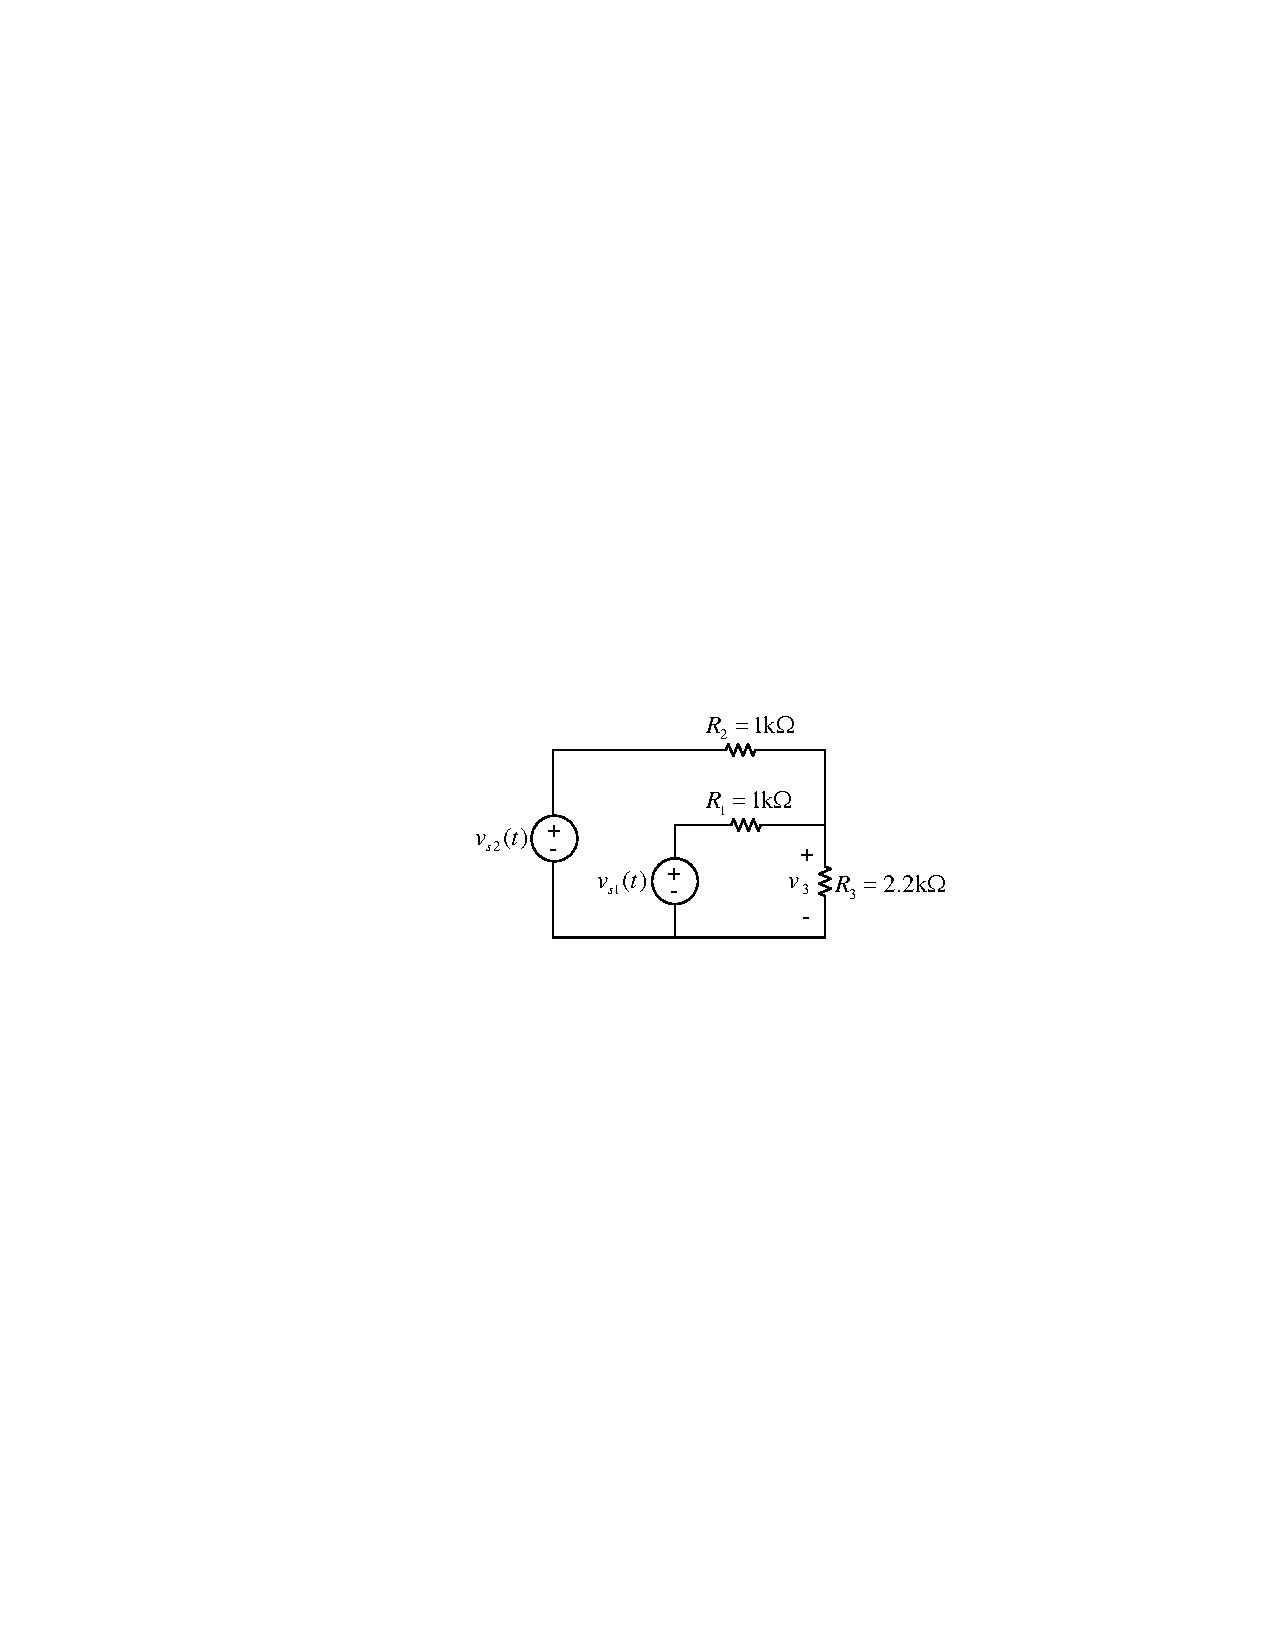
\includegraphics[scale=1.2,angle=0]{Fig/cir1.pdf}
        \caption{A circuit with two voltage sources.} \label{fig:cir1}
    \end{figure}

    %--------------------------------------------
    \begin{subquestion}{Connect $v_{s1}(t)$ and $v_{s2}(t)$ to a $5$V and $10$V DC voltage source, respectively.}
        \answer{
            \begin{figure}[H]
                \centering
                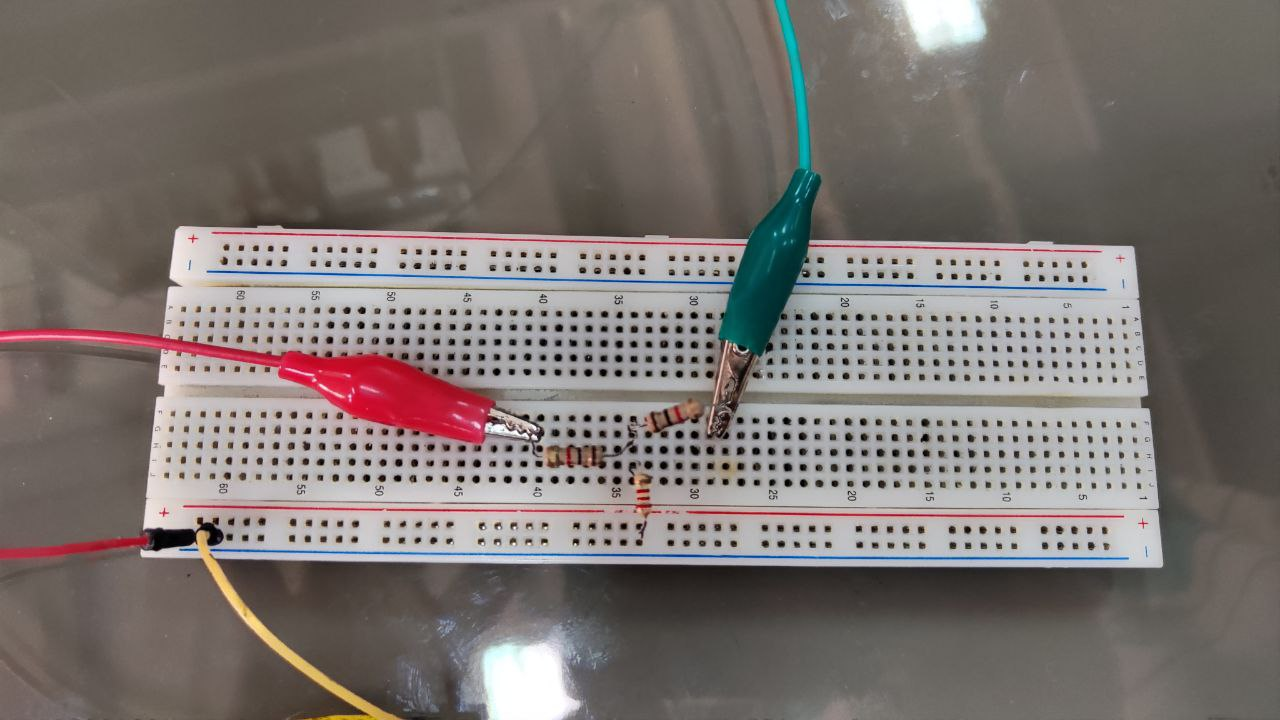
\includegraphics[scale=\PicScale,angle=0]{Fig/1.jpeg}
                \caption{The circuit.}
            \end{figure}
            \begin{figure}[H]
                \centering
                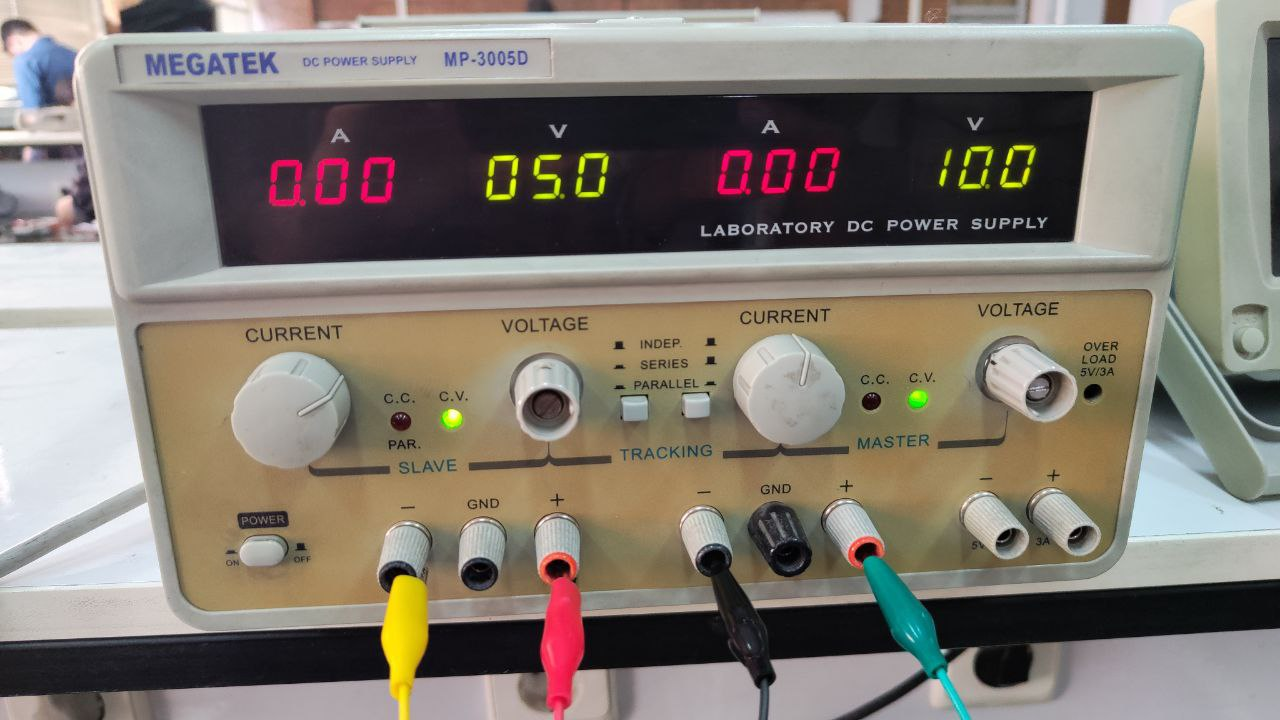
\includegraphics[scale=\PicScale,angle=0]{Fig/2.jpeg}
                \caption{The DC power supply.}
            \end{figure}
        }
    \end{subquestion}

    %--------------------------------------------
    \begin{subquestion}{Measure $v_3$ using a multimeter when $v_{s1}(t)$ is on and $v_{s2}(t)$ is off. Make sure that $v_{s2}(t)$ acts like short circuit when it is off.}
        \answer{
            \begin{figure}[H]
                \centering
                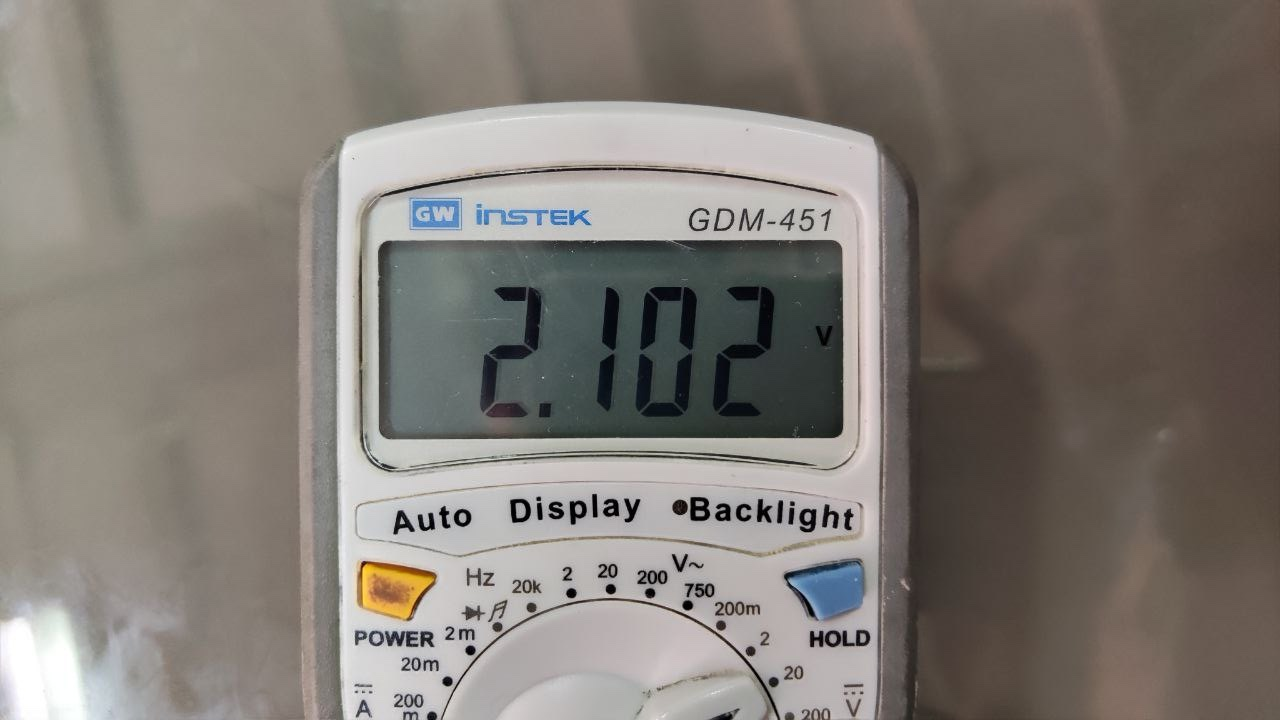
\includegraphics[scale=\PicScale,angle=0]{Fig/3.jpeg}
                % \caption{...}
            \end{figure}
        }
    \end{subquestion}

    %--------------------------------------------
    \begin{subquestion}{Measure $v_3$ using a multimeter when $v_{s2}(t)$ is on and $v_{s1}(t)$ is off. Make sure that $v_{s1}(t)$ acts like short circuit when it is off.}
        \answer{
            \begin{figure}[H]
                \centering
                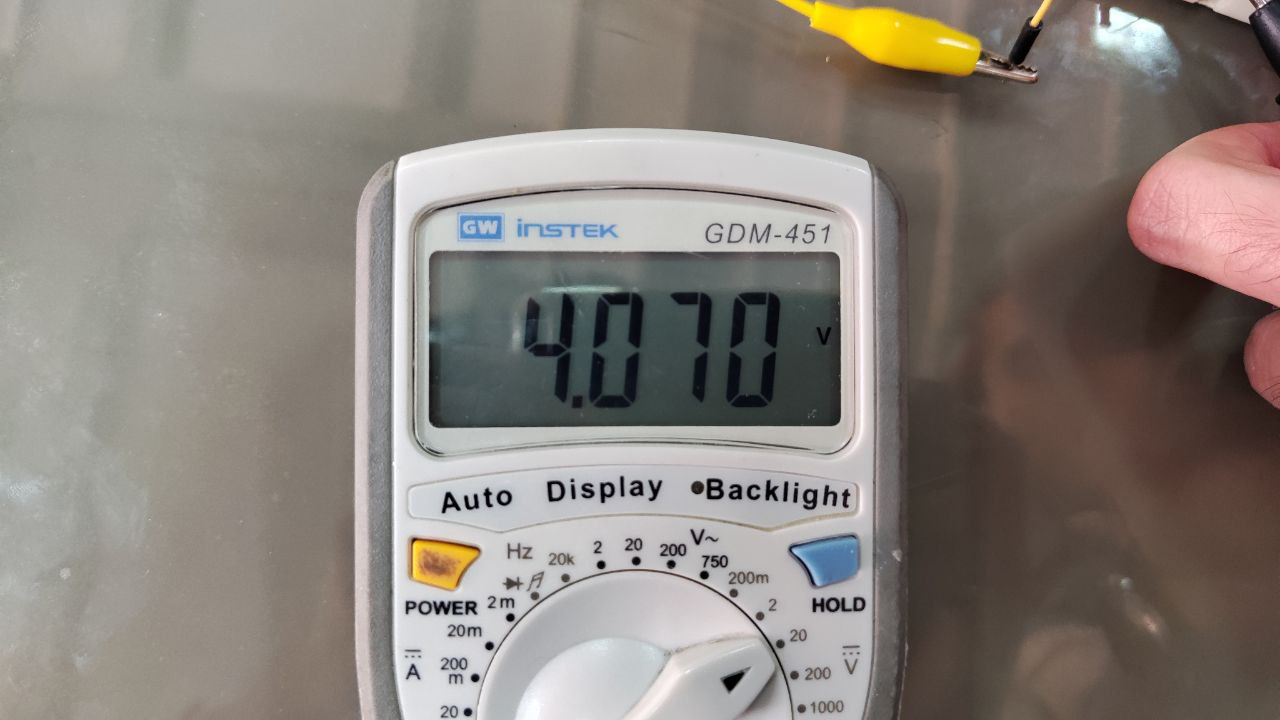
\includegraphics[scale=\PicScale,angle=0]{Fig/4.jpeg}
                % \caption{...}
            \end{figure}
        }
    \end{subquestion}

    %--------------------------------------------
    \begin{subquestion}{Measure $v_3$ using a multimeter when both $v_{s1}(t)$ and $v_{s2}(t)$ are on. Verify the superposition theorem.}
        \answer{
            \begin{figure}[H]
                \centering
                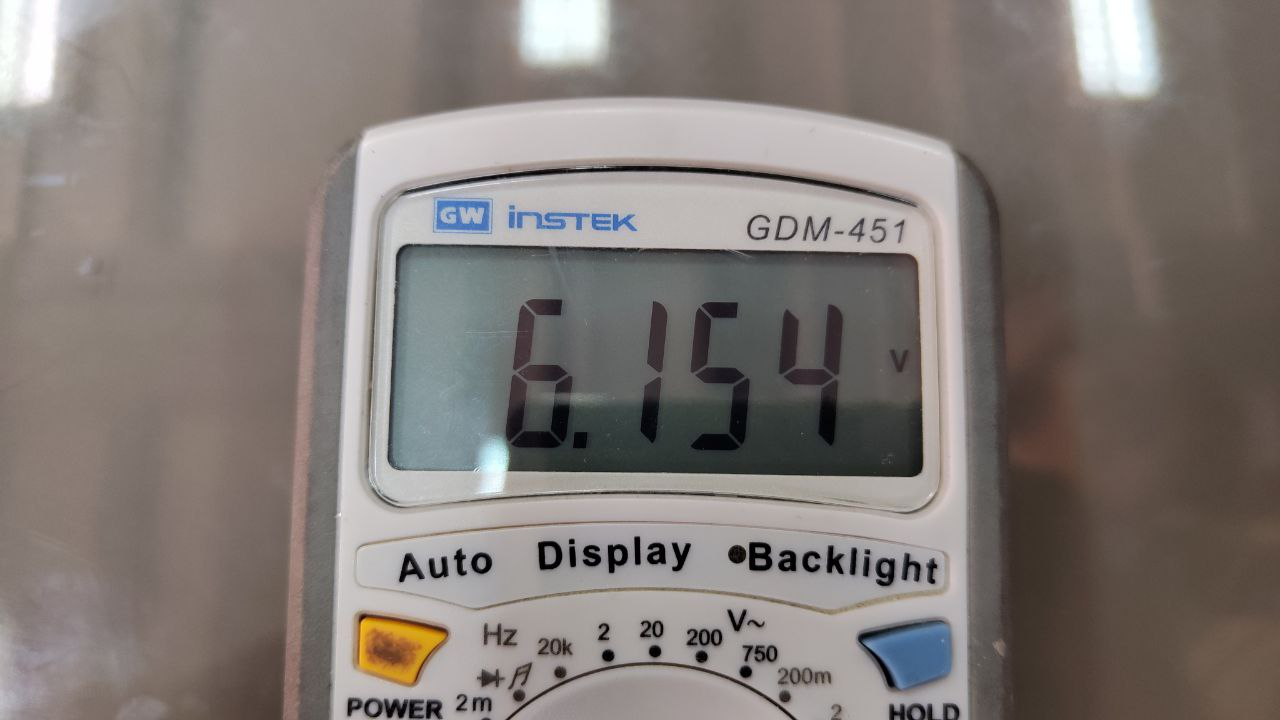
\includegraphics[scale=\PicScale,angle=0]{Fig/5.jpeg}
                % \caption{...}
            \end{figure}
            to verify the superposition theorem, we can use the following equation:
            \begin{equation*}
                v_3 = v_{s1} + v_{s2} = 2.10 + 4.07 = 6.07 \text{ V}
            \end{equation*}
            the direct measure of $v_3$ shows $6.15 V$. So superposition is held in this case, but
            there is about $1.3\%$ error in the measurement.

        }
    \end{subquestion}

    %--------------------------------------------
    \begin{subquestion}{Connect $v_{s1}(t)$ and $v_{s2}(t)$ to a $5$V DC voltage source and a $2$V $1$KHz sine voltage source, respectively. Verify the superposition theorem by suitable measurements using a multimeter. Repeat this part while seeing $v_3$ using an oscilloscope.}
        \answer{
            \begin{figure}[H]
                \centering
                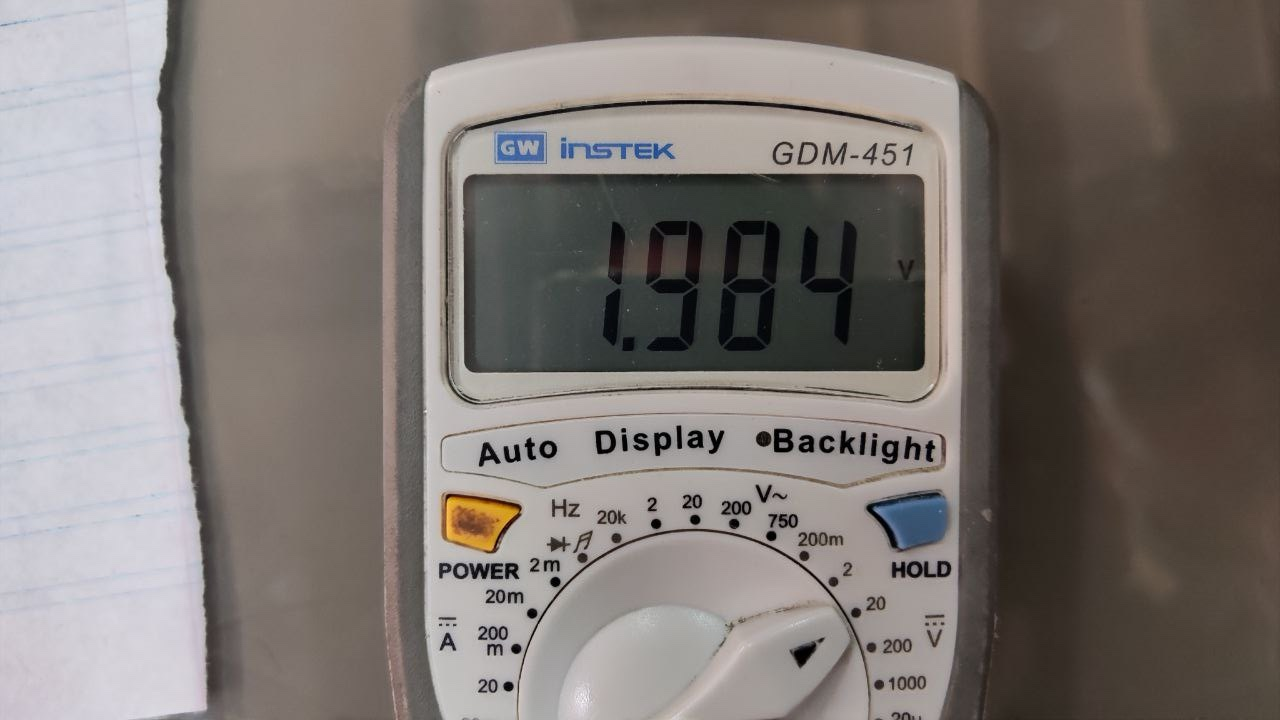
\includegraphics[scale=0.1,angle=0]{Fig/6.jpeg}
                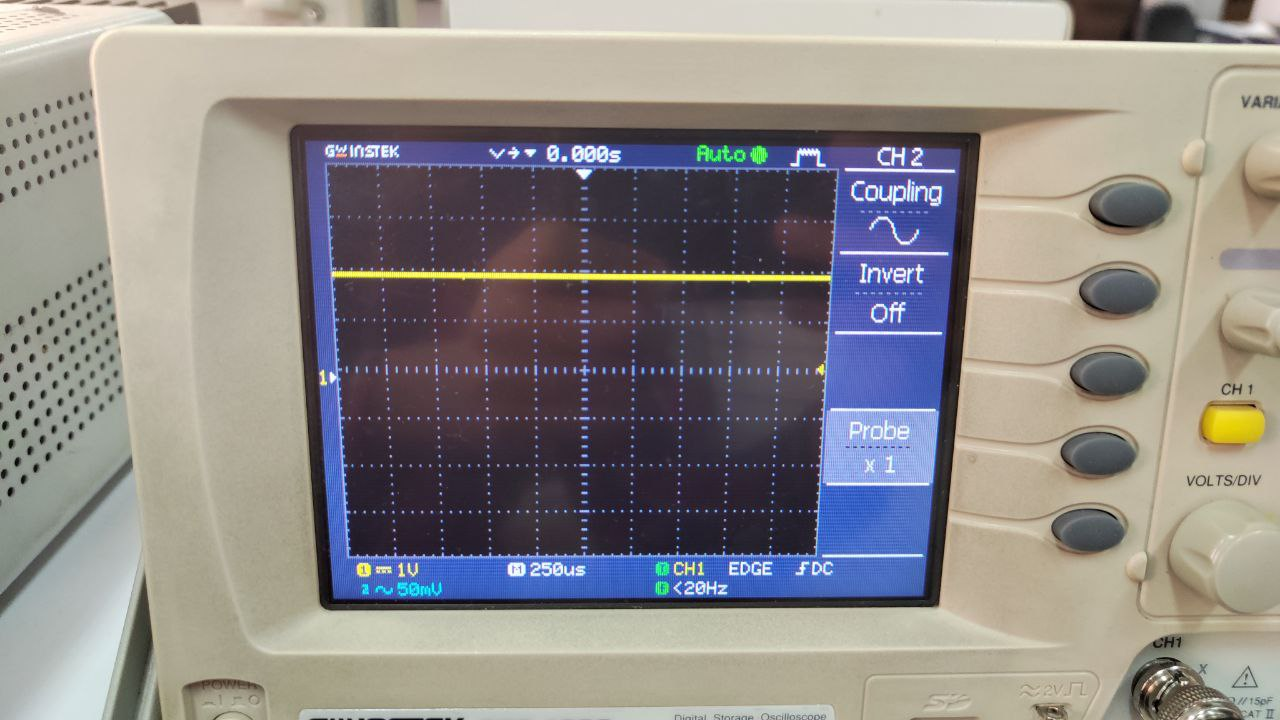
\includegraphics[scale=0.1,angle=0]{Fig/9.jpeg}
                \caption{$v_{s1}$ on and $v_{s2}(t)$ off.}
            \end{figure}
            \begin{figure}[H]
                \centering
                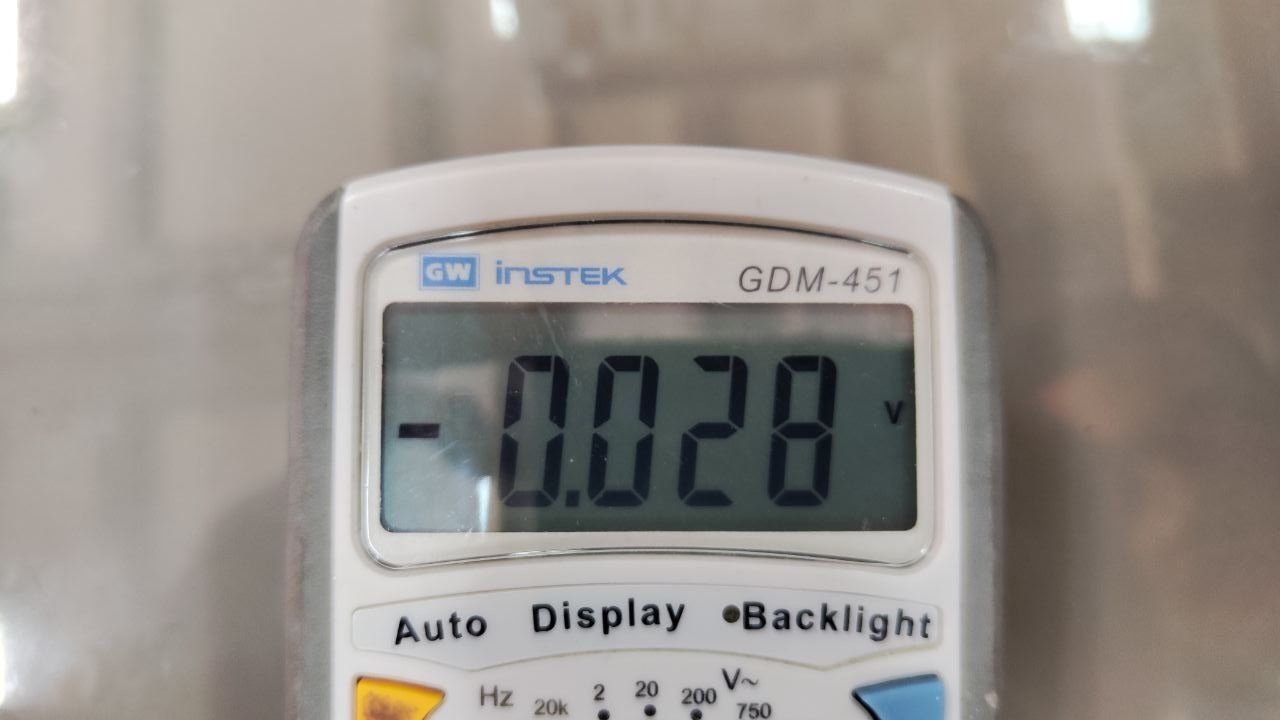
\includegraphics[scale=0.1,angle=0]{Fig/7.jpeg}
                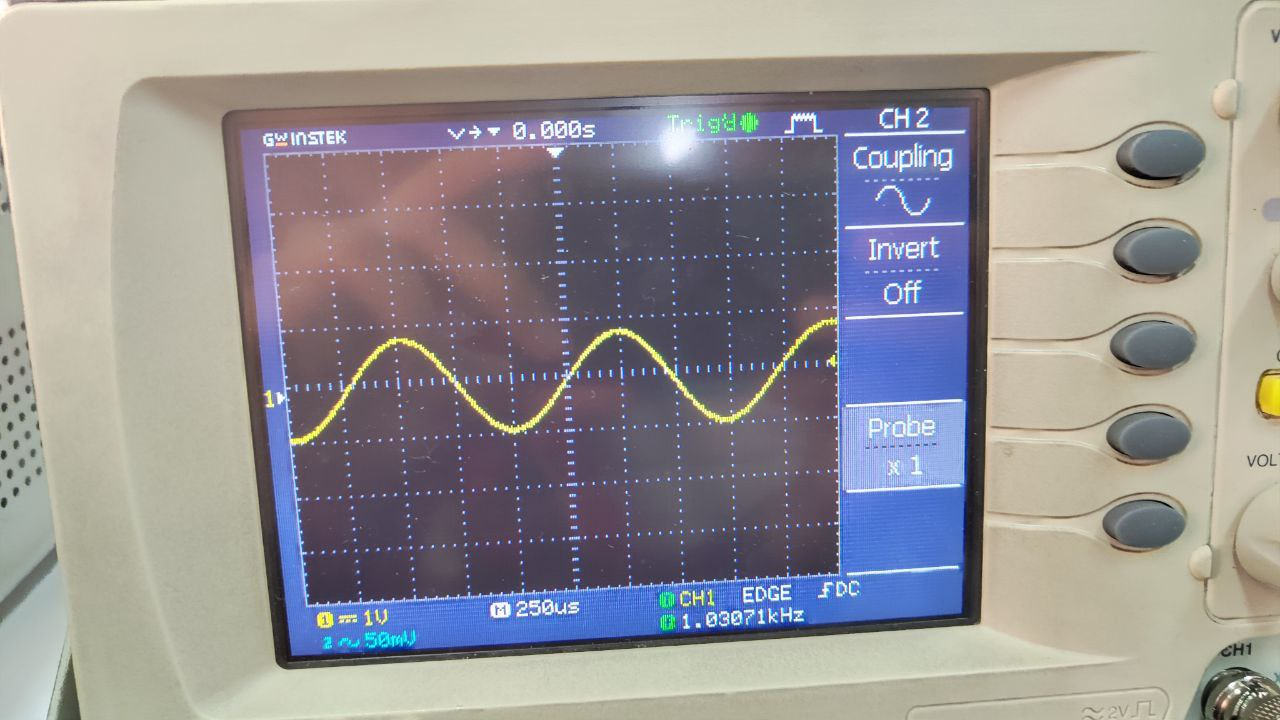
\includegraphics[scale=0.1,angle=0]{Fig/10.jpeg}
                \caption{$v_{s1}$ off and $v_{s2}(t)$ on.}
            \end{figure}
            \begin{figure}[H]
                \centering
                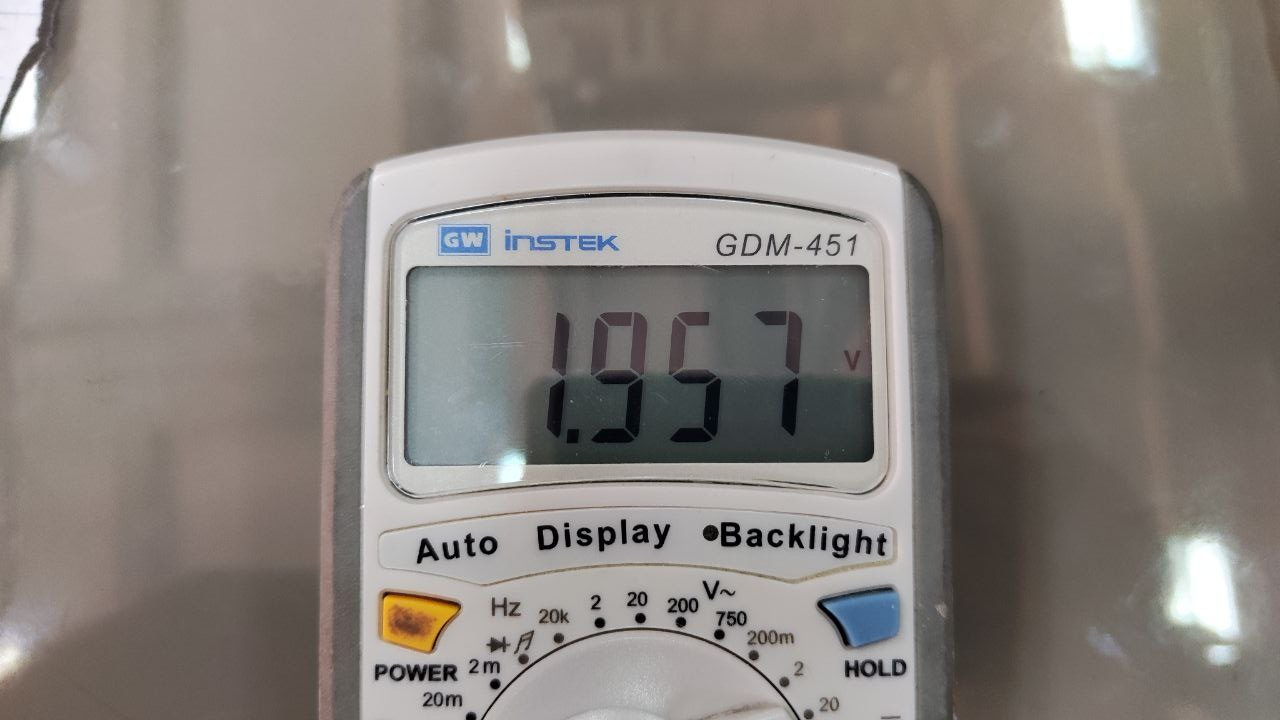
\includegraphics[scale=0.1,angle=0]{Fig/8.jpeg}
                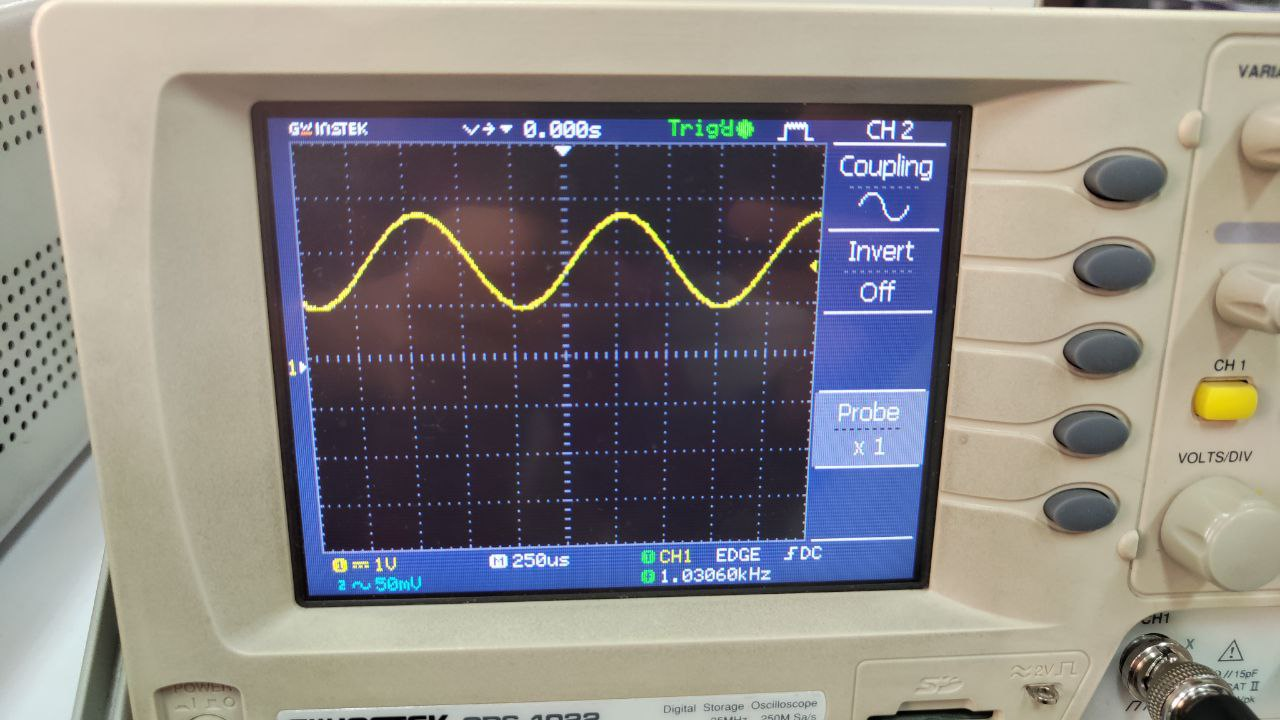
\includegraphics[scale=0.1,angle=0]{Fig/11.jpeg}
                \caption{$v_{s1}$ on and $v_{s2}(t)$ on.}
            \end{figure}

            to verfy superposition, we can use the following equation:
            \begin{equation*}
                v_3 = v_{s1} + v_{s2} = 1.98 - 0.02 = 1.96 \text{ V}
            \end{equation*}
            the direct measure of $v_3$ shows $1.95 V$. So superposition is held in this case, but
            there is about $0.5\%$ error in the measurement.
        }


    \end{subquestion}

    %--------------------------------------------
    \begin{subquestion}{Connect $v_{s1}(t)$ and $v_{s2}(t)$ to a $5$ V and $10$ V DC voltage source, respectively, and replace $R_1$ and $R_2$ with two diodes such that the positive leg of each diode connects to the positive side of the corresponding voltage source. Check if the superposition is held or not. Discuss the results.}
        \answer{
            \begin{figure}[H]
                \centering
                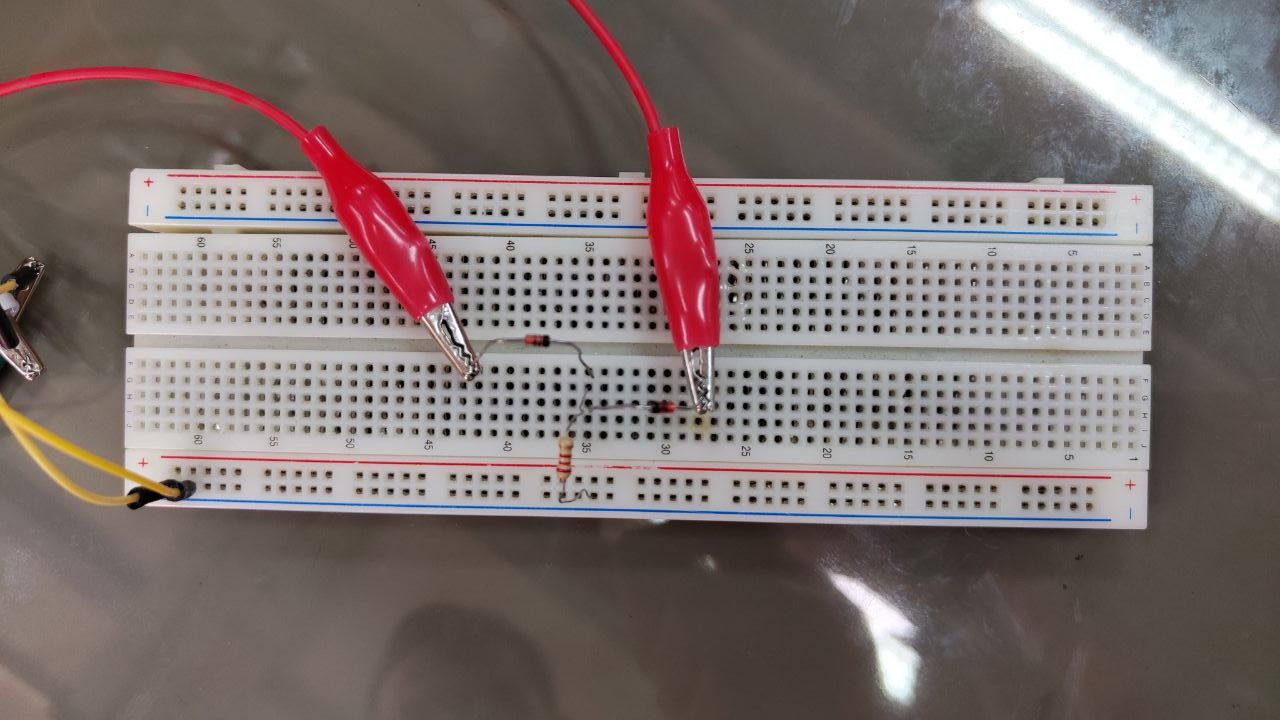
\includegraphics[scale=\PicScale,angle=0]{Fig/12.jpeg}
                \caption{The circuit.}
            \end{figure}
            \begin{figure}[H]
                \centering
                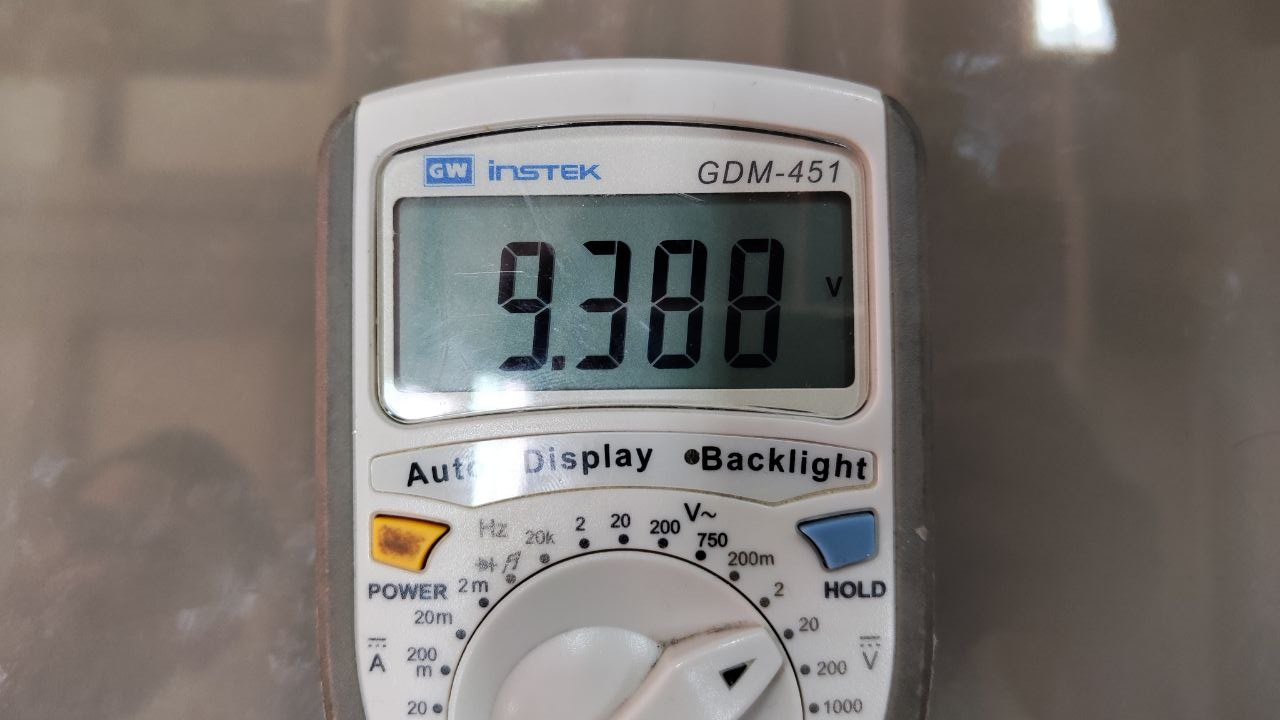
\includegraphics[scale=\PicScale,angle=0]{Fig/13.jpeg}
                \caption{$v_{s1}$ on and $v_{s2}(t)$ off.}
            \end{figure}
            \begin{figure}[H]
                \centering
                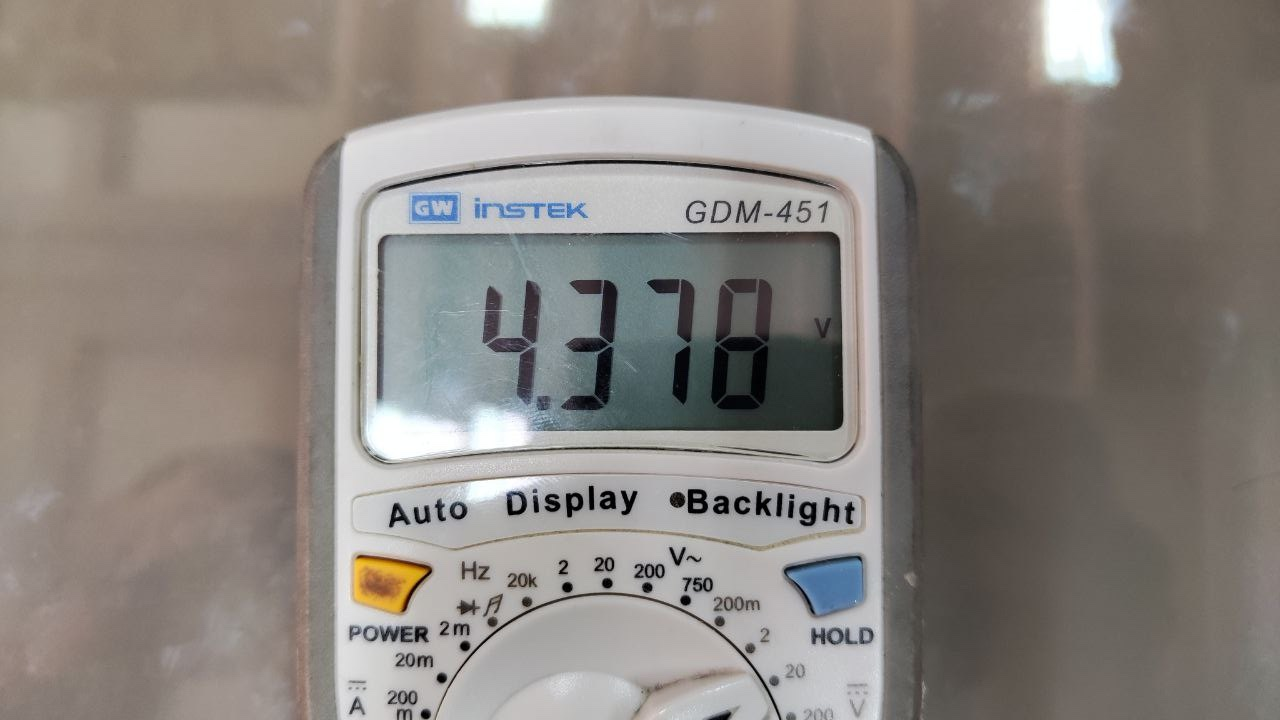
\includegraphics[scale=\PicScale,angle=0]{Fig/14.jpeg}
                \caption{$v_{s1}$ off and $v_{s2}(t)$ on.}
            \end{figure}
            \begin{figure}[H]
                \centering
                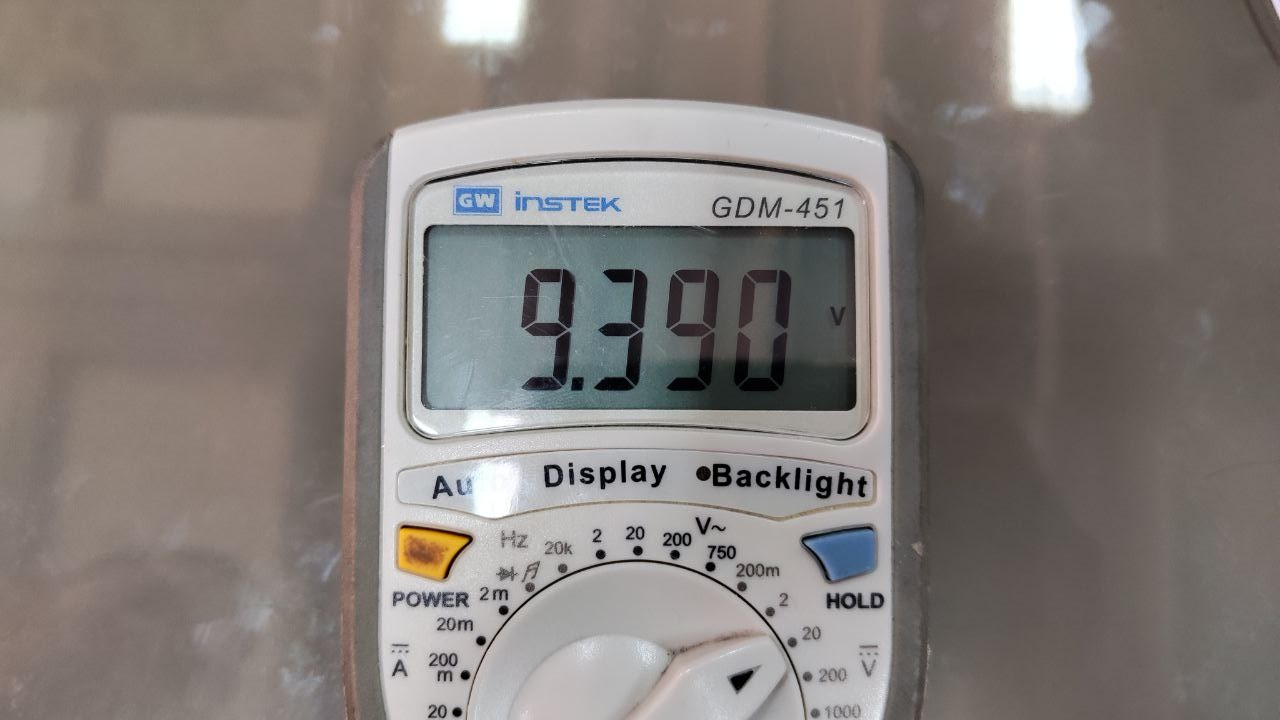
\includegraphics[scale=\PicScale,angle=0]{Fig/15.jpeg}
                \caption{$v_{s1}$ on and $v_{s2}(t)$ on.}
            \end{figure}

            Since diode is considered as a non-linear element,
            the superposition theorem is not held in this case and
            $v_3$ is not equal to the sum of $v_{s1}$ and $v_{s2}$.
        }
    \end{subquestion}

\end{question}

%----------------------------------------------------------------------------------------
%	QUESTION 2
%----------------------------------------------------------------------------------------

\begin{question}

    \questiontext{Build the circuit shown in Fig. \ref{fig:cir2} on a breadboard.}

    \begin{figure}[H]
        \centering
        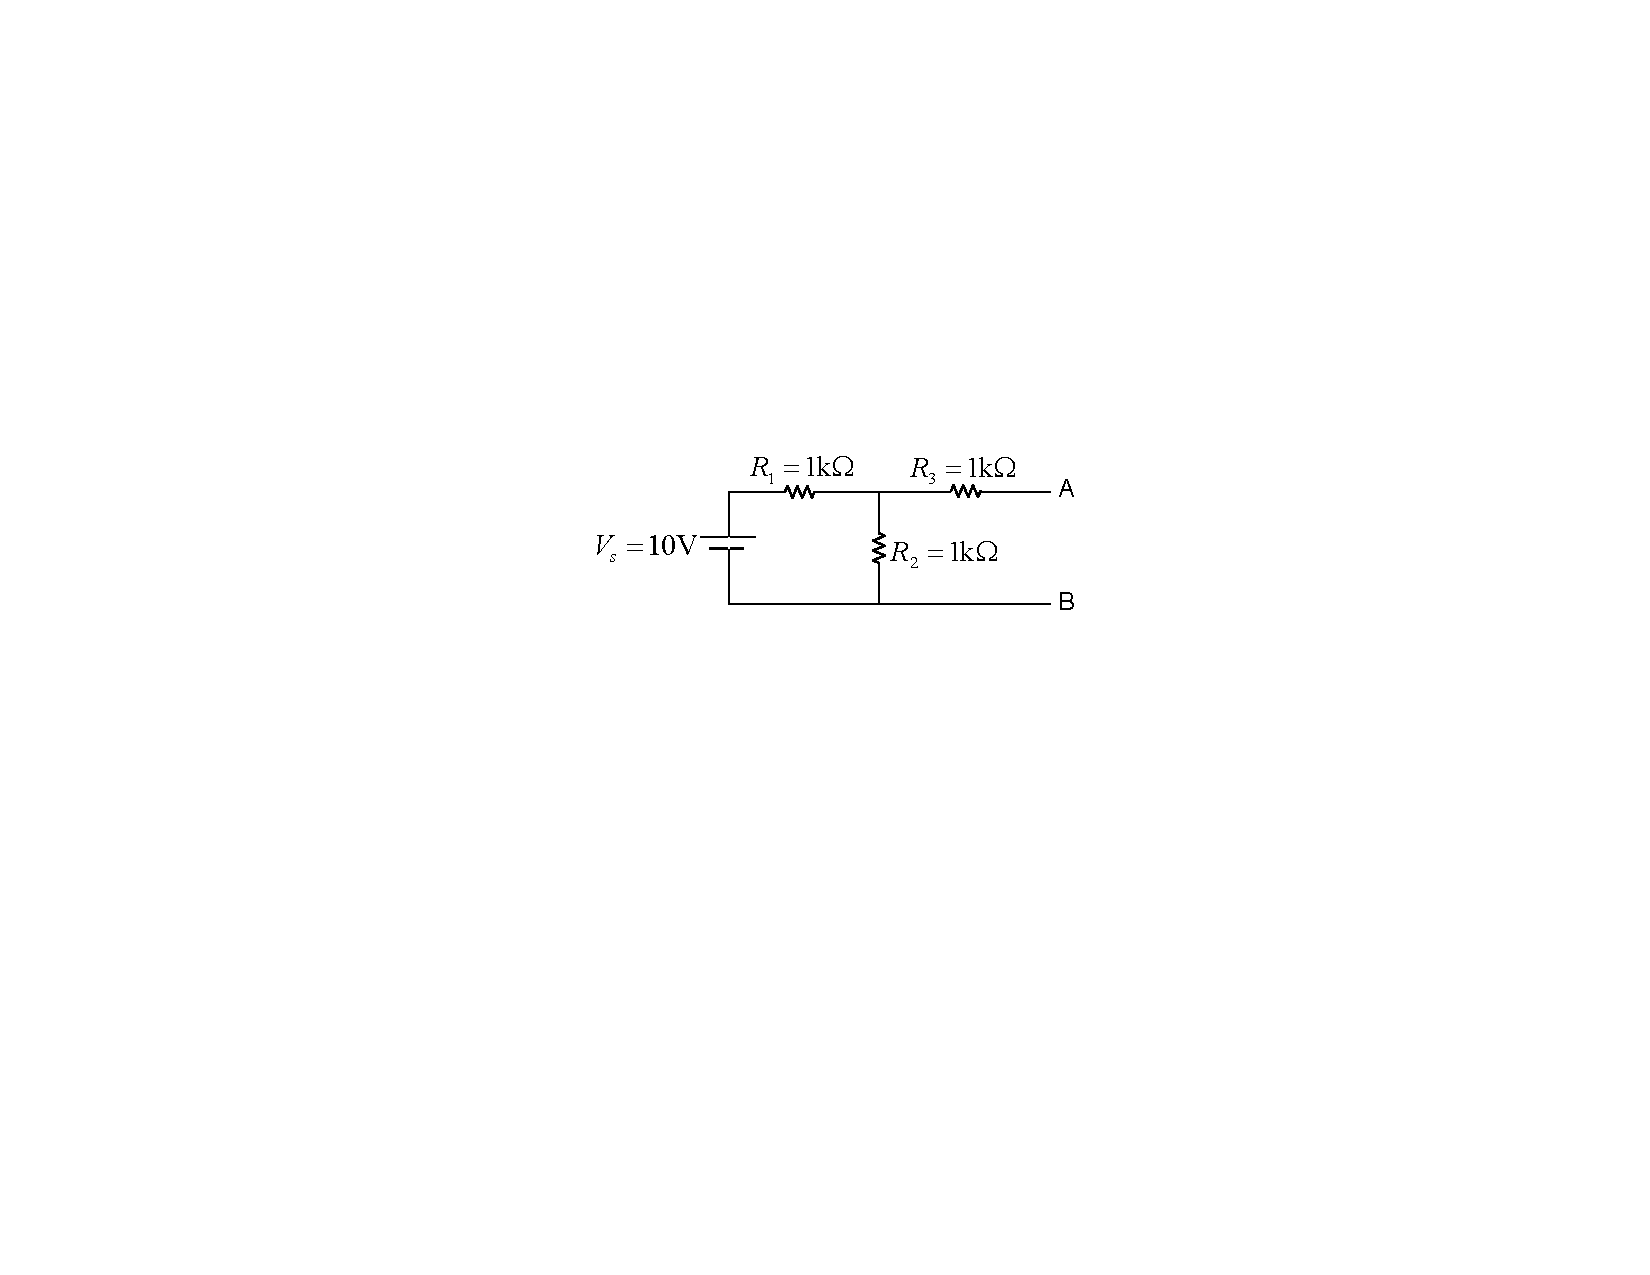
\includegraphics[scale=1.2,angle=0]{Fig/cir2.pdf}
        \caption{A linear circuit.} \label{fig:cir2}
    \end{figure}


    %--------------------------------------------
    \begin{subquestion}{Measure the open circuit voltage $V_{oc}$ of the circuit.}
        \answer{
            \begin{figure}[H]
                \centering
                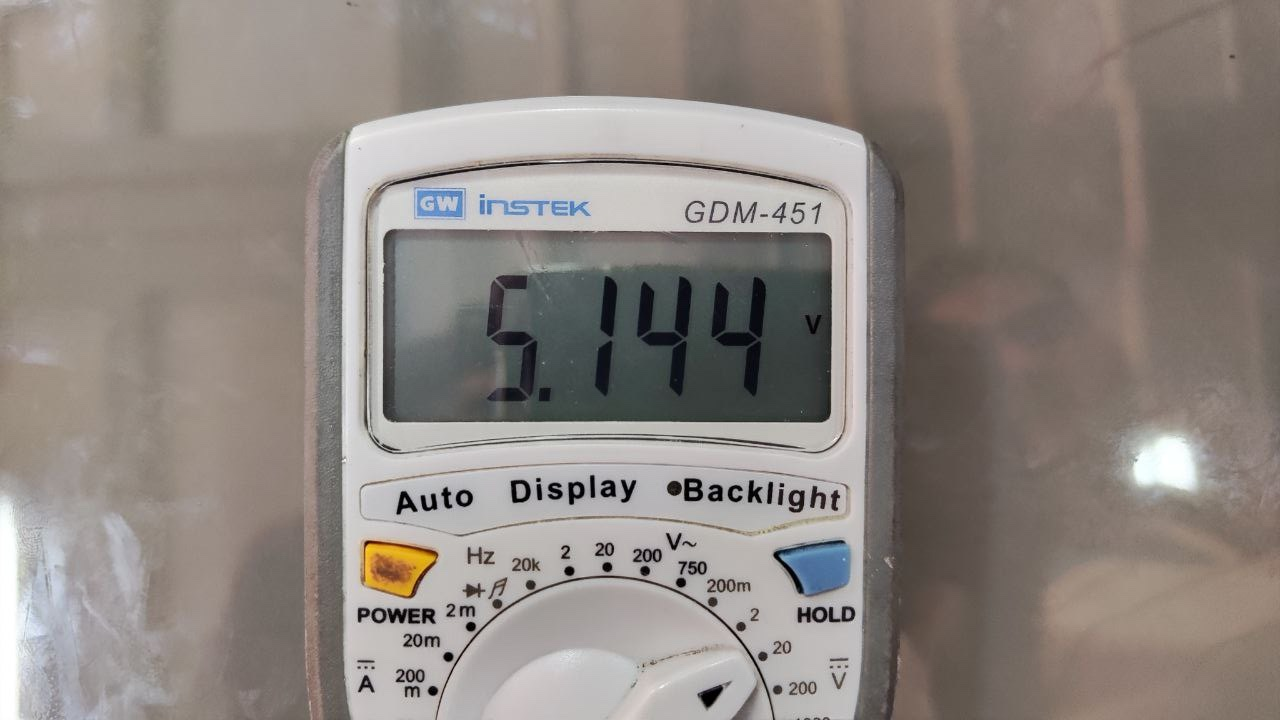
\includegraphics[scale=\PicScale,angle=0]{Fig/16.jpeg}
                % \caption{...}
            \end{figure}
        }
    \end{subquestion}

    %--------------------------------------------
    \begin{subquestion}{Connect an $R_L=2.2$ k$\Omega$ resistor to the port AB and measure its voltage $V_L$.}
        \answer{
            \begin{figure}[H]
                \centering
                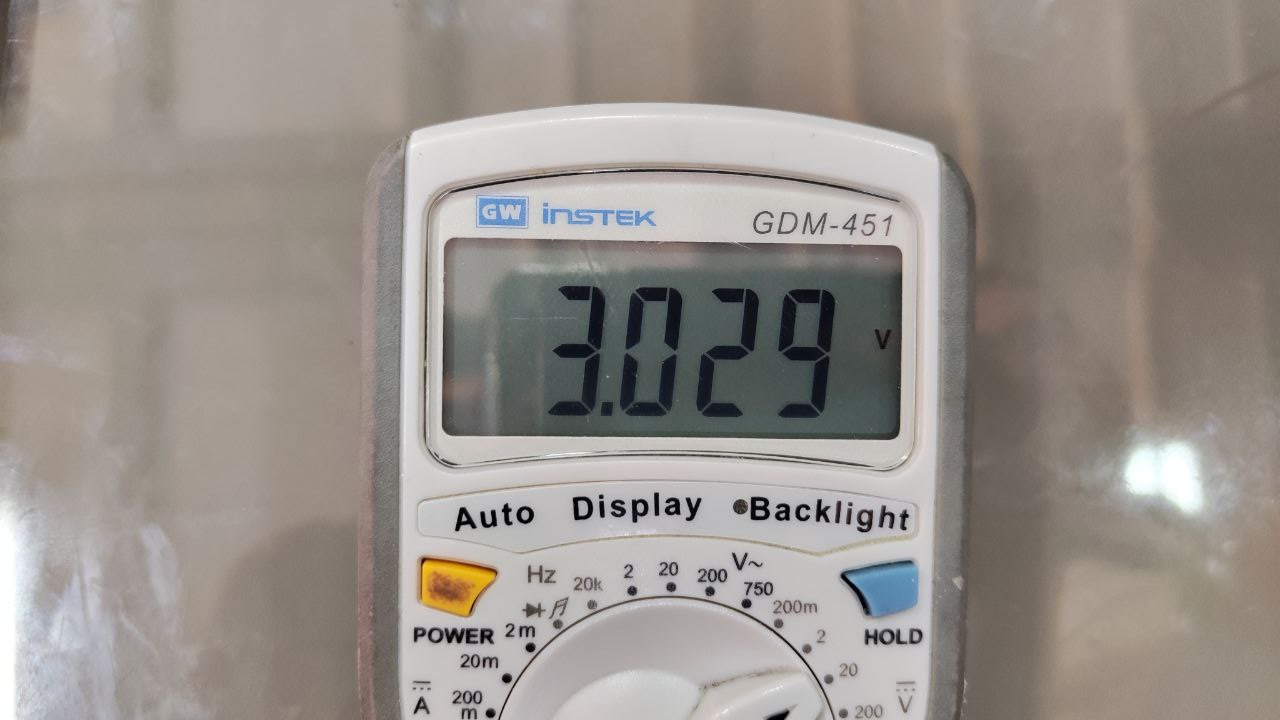
\includegraphics[scale=\PicScale,angle=0]{Fig/17.jpeg}
                % \caption{...}
            \end{figure}
        }
    \end{subquestion}

    %--------------------------------------------
    \begin{subquestion}{Can you obtain the corresponding Thevenin equivalent circuit using the measured values of $V_{oc}$ and $V_L$.}
        \answer{
            % \begin{figure}[H]
            %     \centering
            %     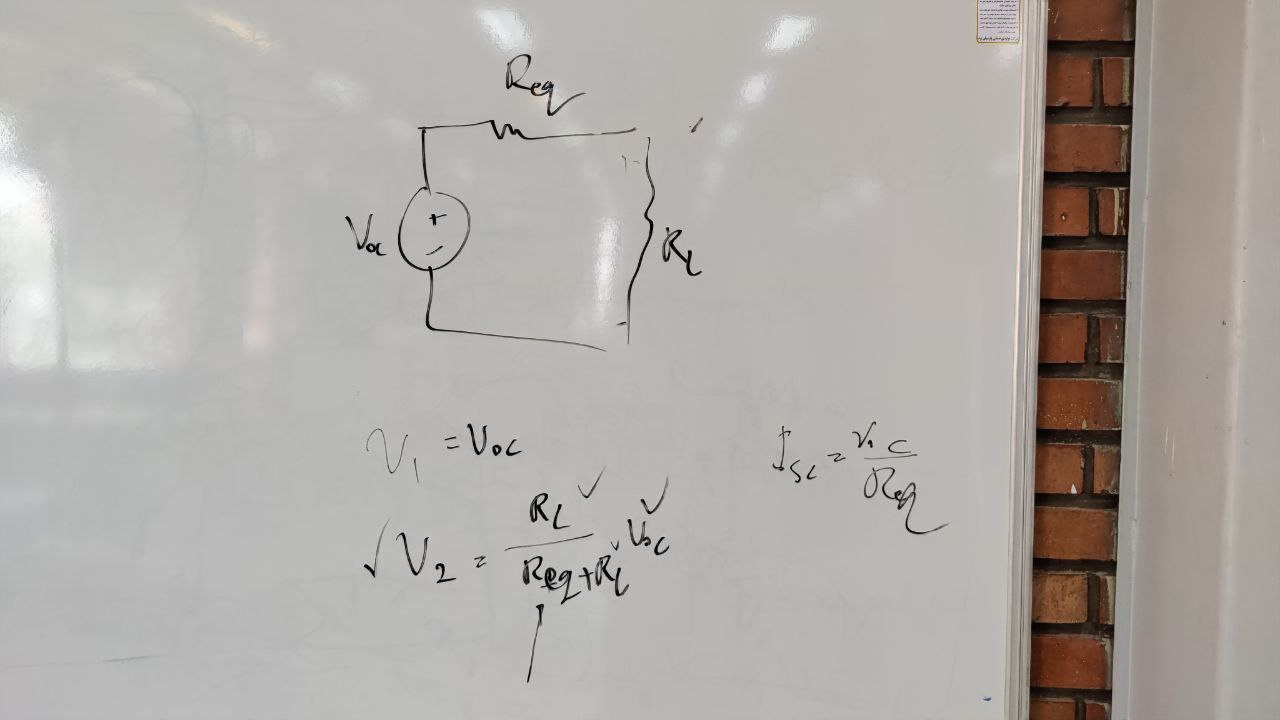
\includegraphics[scale=\PicScale,angle=0]{Fig/123456789.jpeg}
            %     \caption{its just for you to help you to write this part. delete it in final version.}
            % \end{figure}

            Considering a series circuit which contains voltage source $V_{oc}$ , $R_{eq}$
            and $R_L$, the relation between variables of this circuit and the original circuit is:
            \begin{equation*}
                V_{oc} = V_{1} \quad V_{L} = \frac{R_L}{R_{eq}+R_L} \times V_{oc} \quad I_{sc} = \frac{V_{oc}}{R_{eq}}
            \end{equation*}

            Using the equations, since $V_{oc} = 5.14$ V and $V_{L} = 3.02$ V
            and $R_L = 2.2$ k$\Omega$, we can find $R_{eq}$ as:
            \begin{equation*}
                R_{eq} = 1.56 \text{ k}\Omega
            \end{equation*}
            So the Thevenin equivalent circuit is a voltage source with $V_{oc} = 5.14$ V and
            a resistor with $R_{eq} = 1.56$ k$\Omega$.
        }
    \end{subquestion}

    %--------------------------------------------
    \begin{subquestion}{Build the Thevenin equivalent circuit on the breadboard. Connect a same load resistor to both circuits and measure its voltage. Interpret the results.}
        \answer{
            \begin{figure}[H]
                \centering
                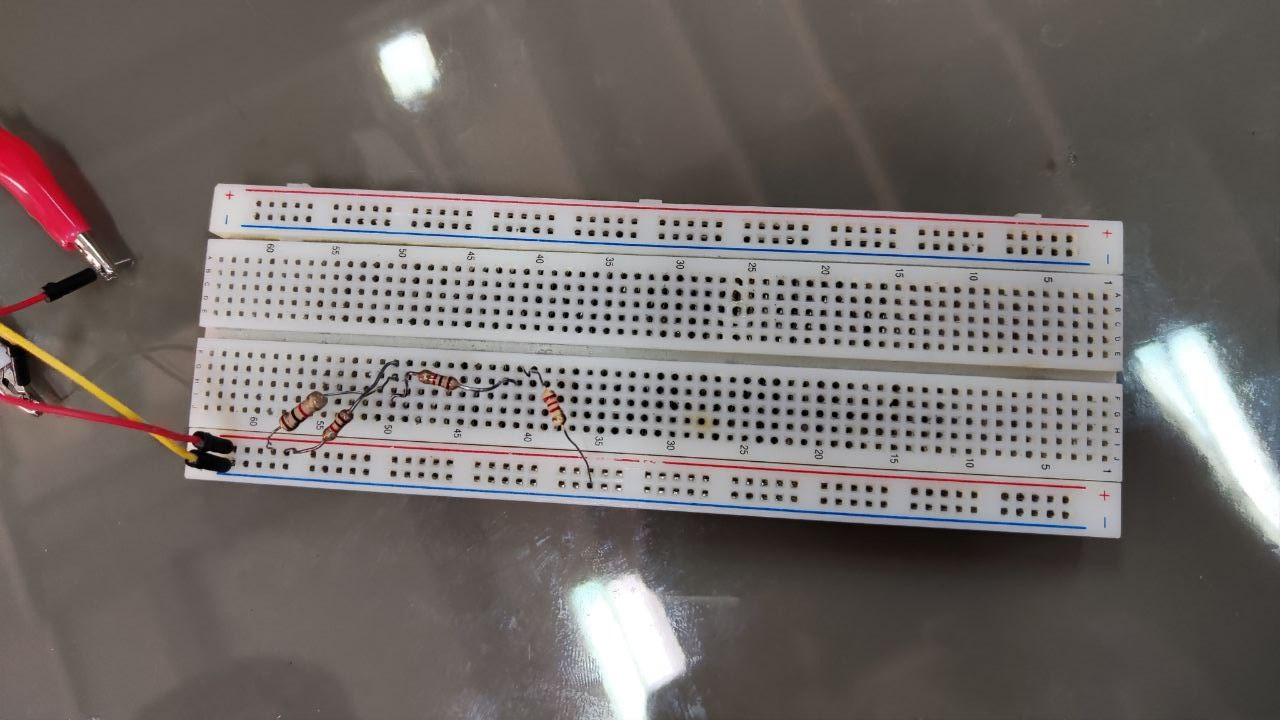
\includegraphics[scale=\PicScale,angle=0]{Fig/18.jpeg}
                \caption{The circuit.}
            \end{figure}
            \begin{figure}[H]
                \centering
                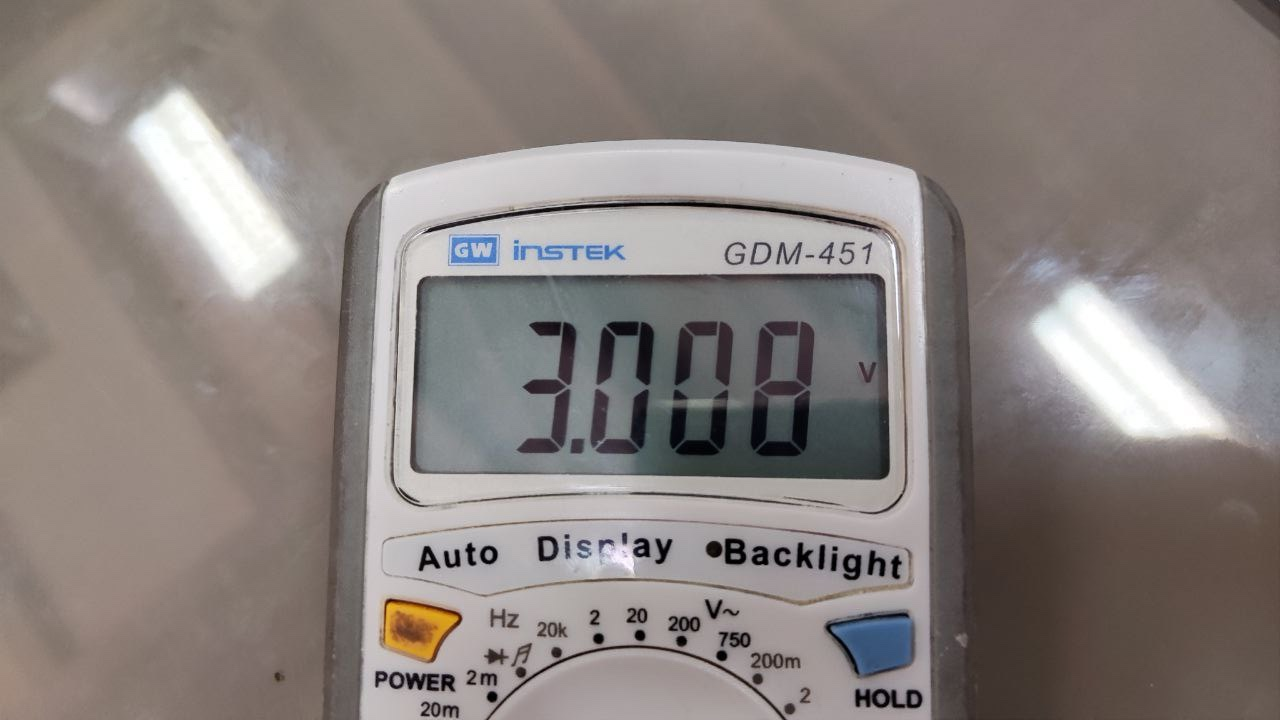
\includegraphics[scale=\PicScale,angle=0]{Fig/19.jpeg}
                \caption{Voltage of the load resistor.}
            \end{figure}

            The voltage of the load resistor is $3.00$ V which has a $0.7\%$ error.
            This can be due to tolerances of the components (like resistors).
        }
    \end{subquestion}

\end{question}


%----------------------------------------------------------------------------------------
%	QUESTION 3
%----------------------------------------------------------------------------------------

\begin{question}

    \questiontext{Build the circuit shown in Fig. \ref{fig:cir3} on a breadboard.}

    \begin{figure}[H]
        \centering
        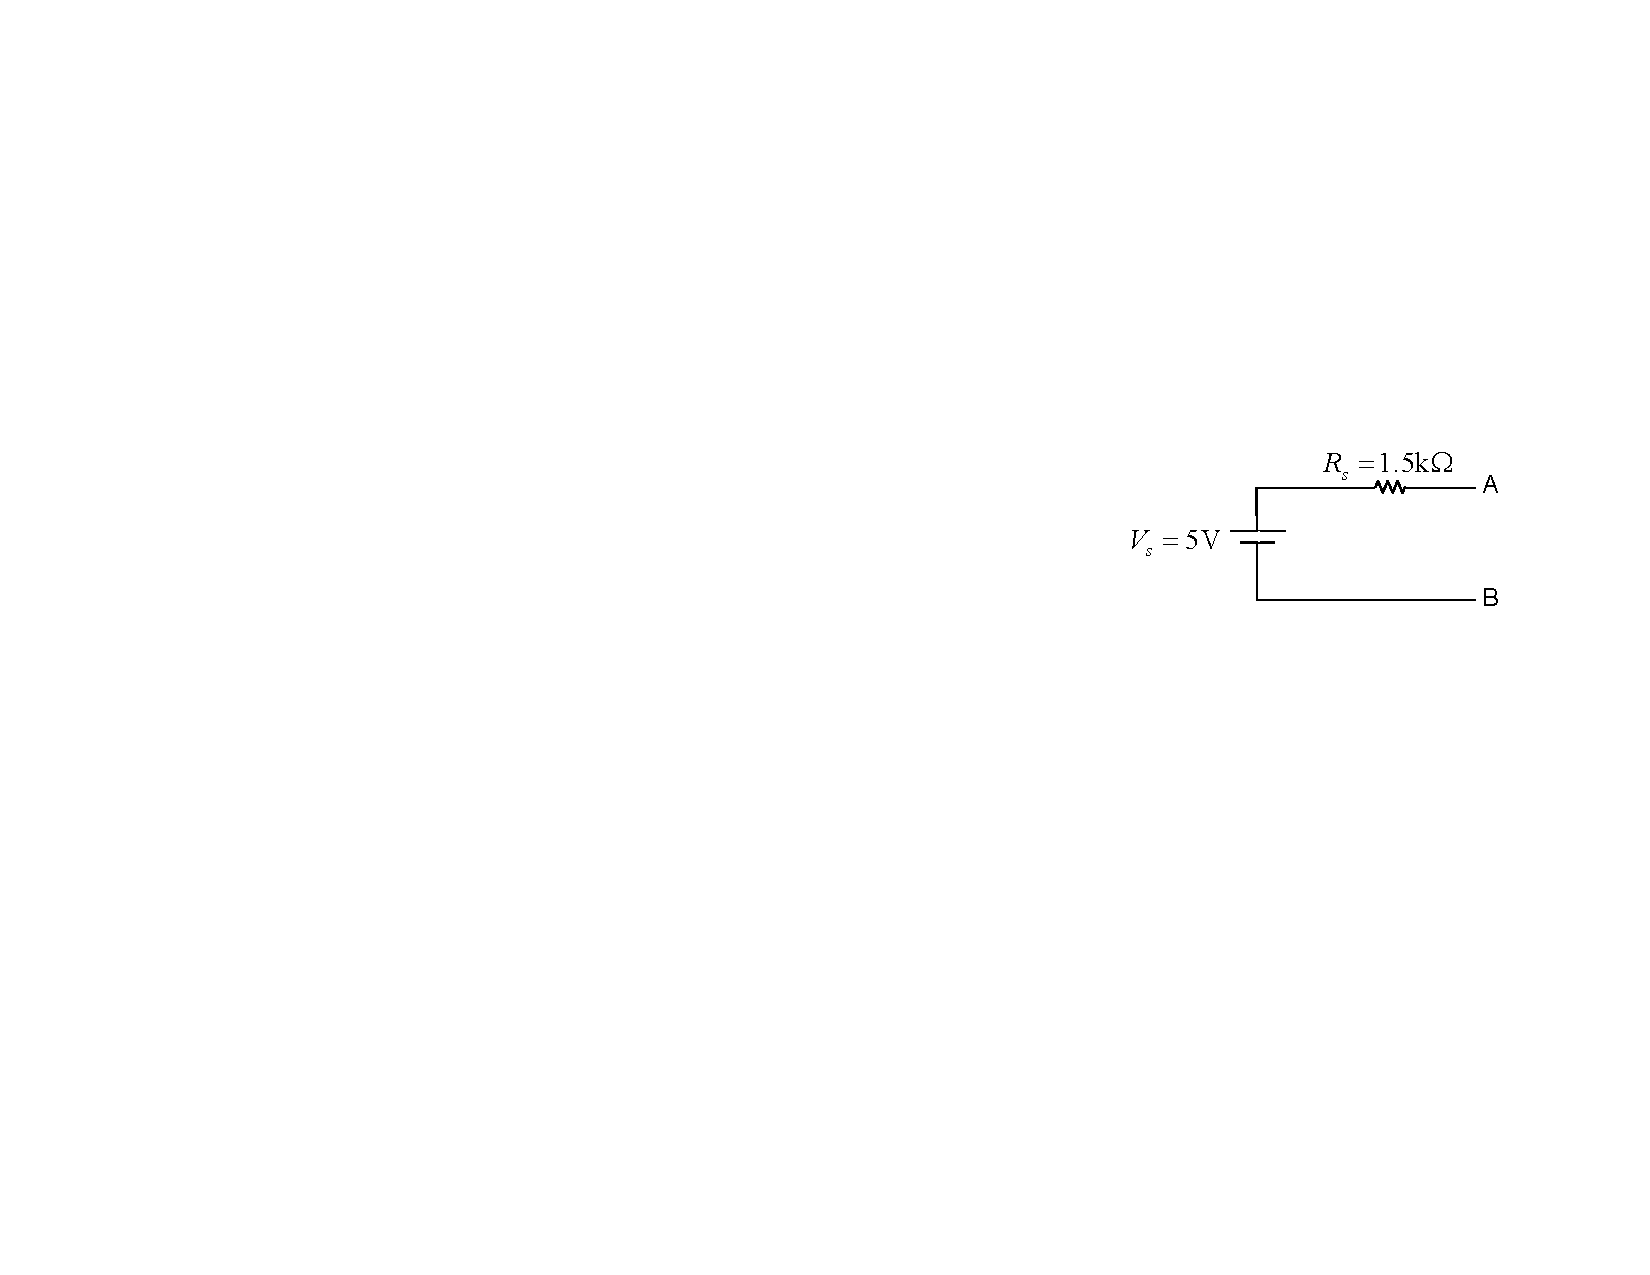
\includegraphics[scale=1.2,angle=0]{Fig/cir3.pdf}
        \caption{A simple resistive circuit.} \label{fig:cir3}
    \end{figure}


    %--------------------------------------------
    \begin{subquestion}{Calculate the load resistor $R_L$ drawing the maximum power from the source. Connect it to the port AB and measure the consumed power.}
        \answer{
            \begin{figure}[H]
                \centering
                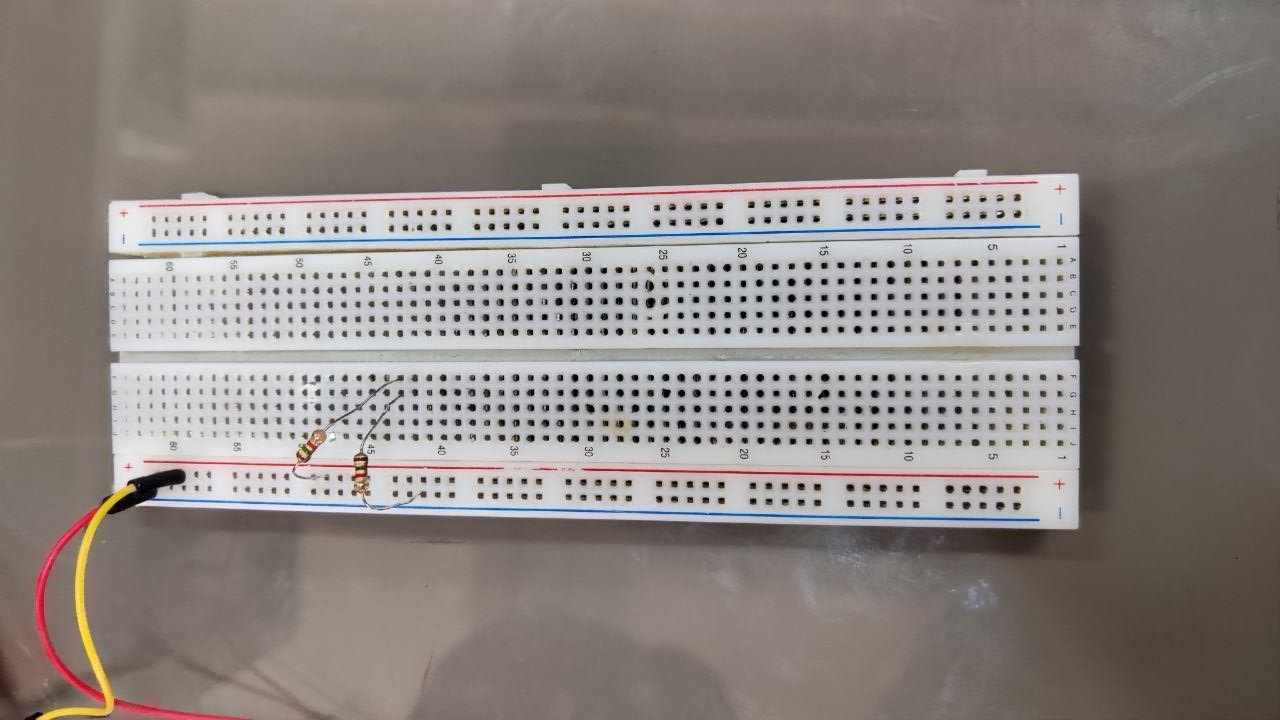
\includegraphics[scale=\PicScale,angle=0]{Fig/20.jpeg}
                \caption{The circuit.}
            \end{figure}
            \begin{figure}[H]
                \centering
                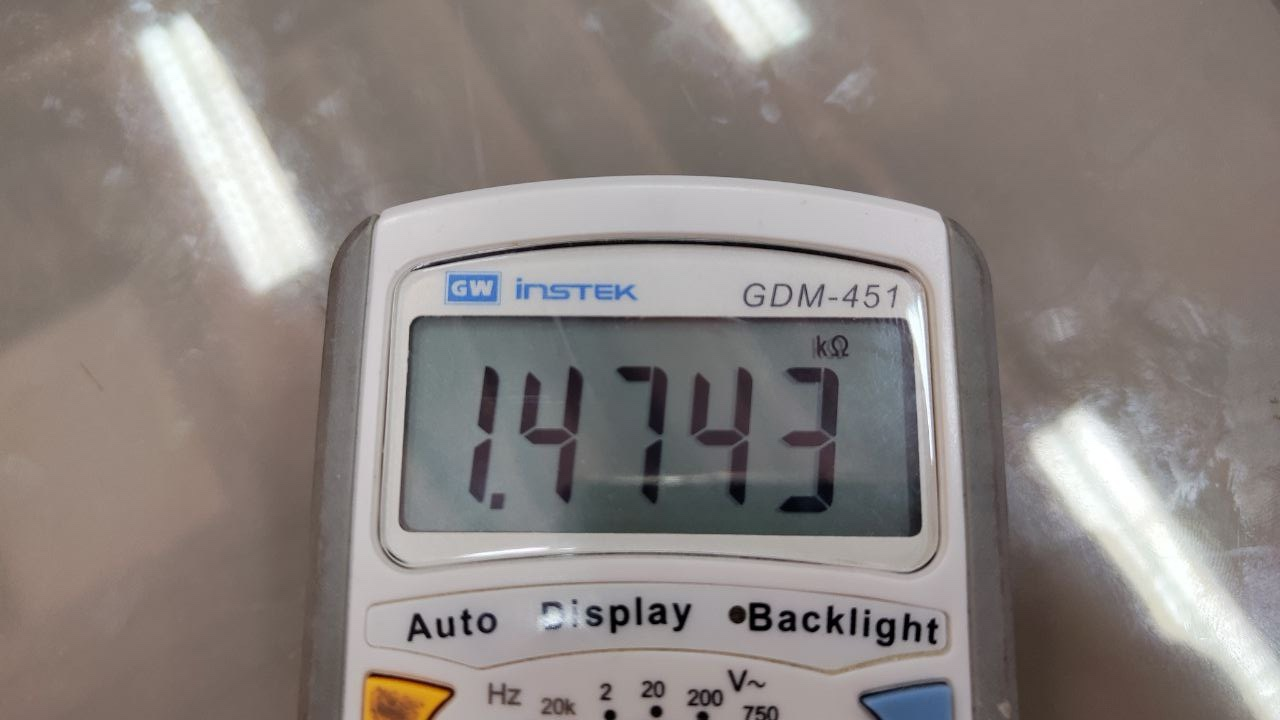
\includegraphics[scale=\PicScale,angle=0]{Fig/21.jpeg}
                \caption{The exact value of $R$.}
            \end{figure}
            \begin{figure}[H]
                \centering
                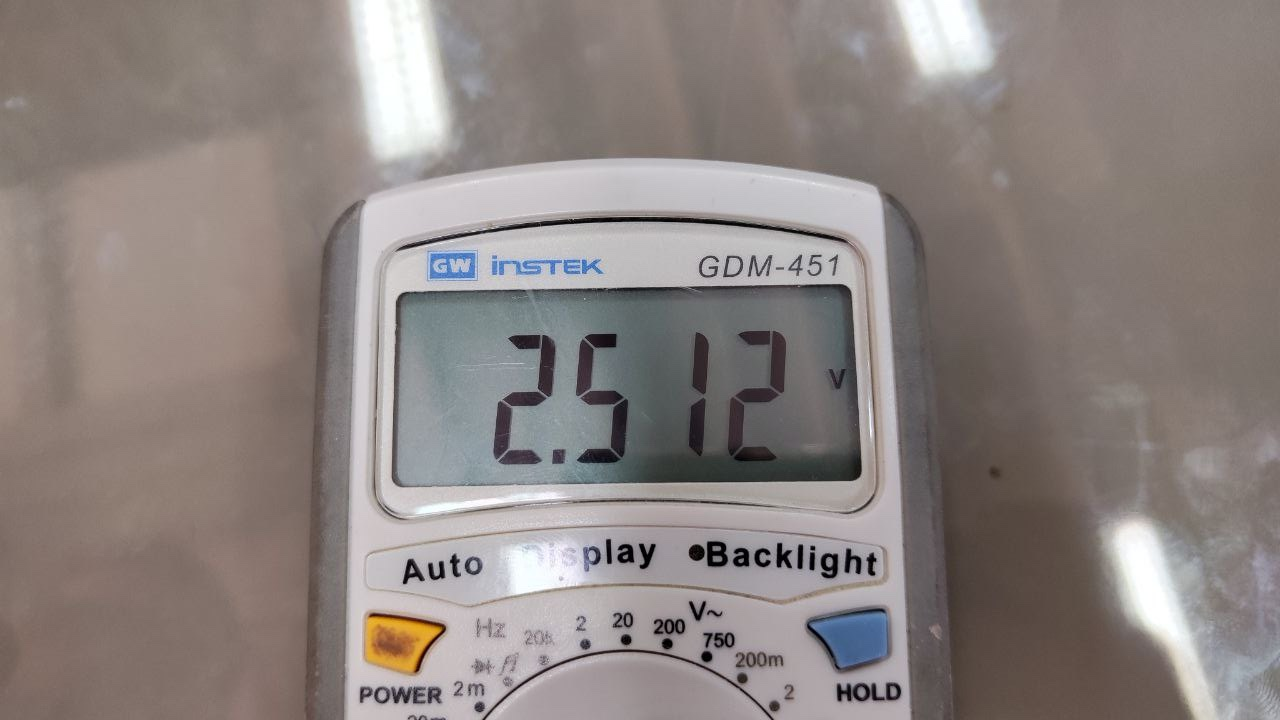
\includegraphics[scale=\PicScale,angle=0]{Fig/22.jpeg}
                \caption{The exact value of $v$ of $R$.}
            \end{figure}

            The power consumed will be maximum when $R_L = R_{eq} = 1.45$ k$\Omega$.
            Using $\frac{V^2}{R}$ for calculation of power, we will have:
            \begin{equation*}
                P = \frac{v^2}{R} = \frac{2.51^2}{1.45} = 4.35 \text{ W}
            \end{equation*}
        }
    \end{subquestion}

    %--------------------------------------------
    \begin{subquestion}{Connect a $1$ k$\Omega$ and a $2.2$ k$\Omega$ resistor to the port and measure the corresponding consumed powers. Discuss the results and verify the maximum power transfer theorem.}
        \answer{
            \begin{figure}[H]
                \centering
                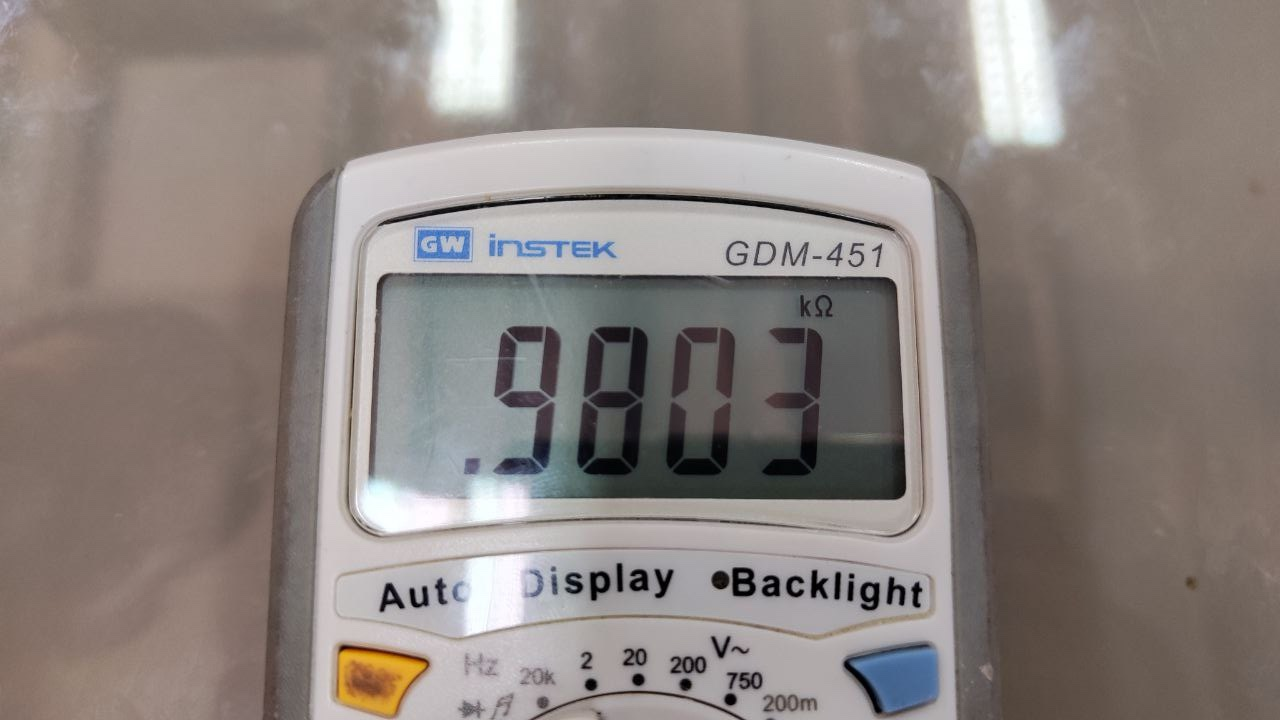
\includegraphics[scale=\PicScale,angle=0]{Fig/23.jpeg}
                \caption{The exact value of $R$.}
            \end{figure}
            \begin{figure}[H]
                \centering
                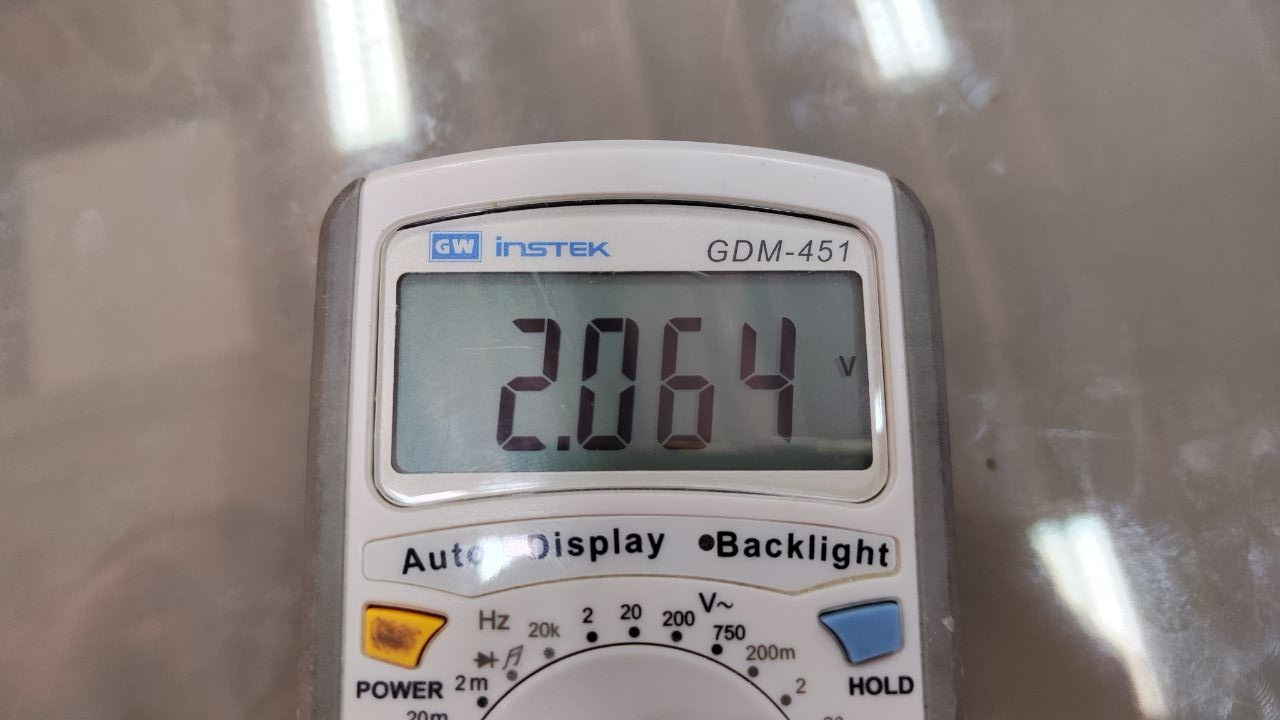
\includegraphics[scale=\PicScale,angle=0]{Fig/24.jpeg}
                \caption{The exact value of $v$ of $R=0.98k$.}
            \end{figure}
            \begin{figure}[H]
                \centering
                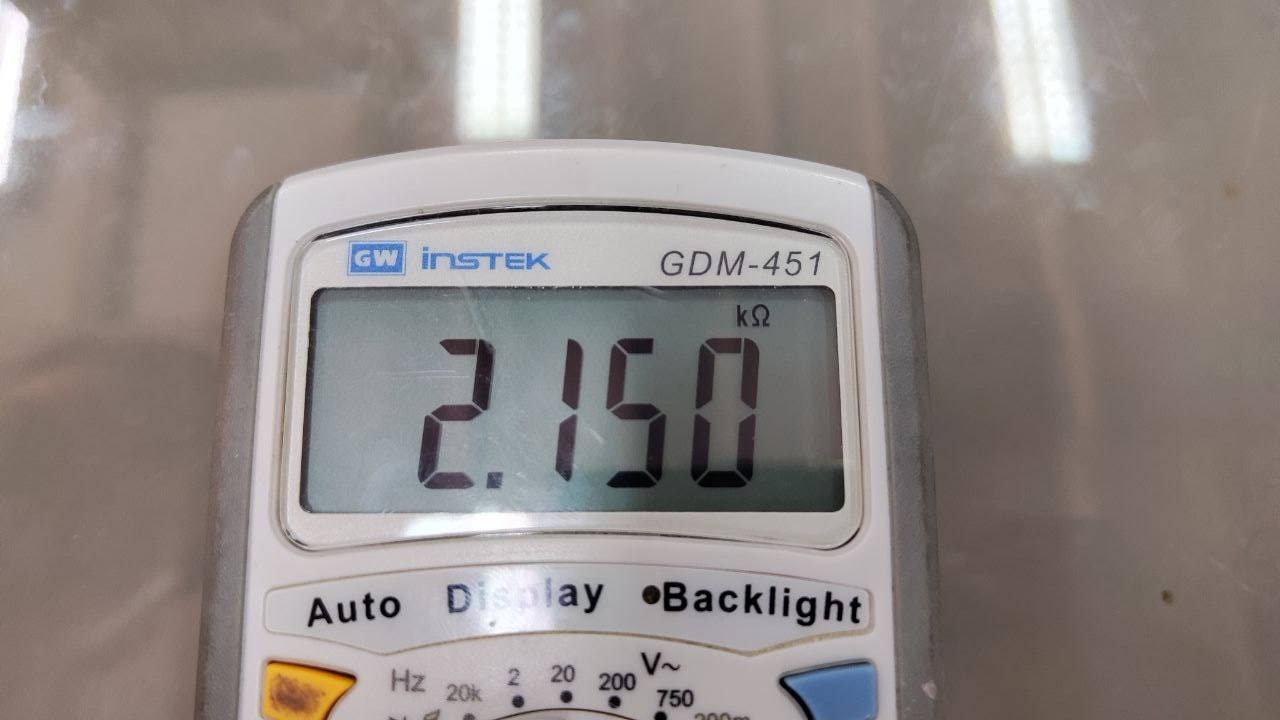
\includegraphics[scale=\PicScale,angle=0]{Fig/25.jpeg}
                \caption{The exact value of $R$.}
            \end{figure}
            \begin{figure}[H]
                \centering
                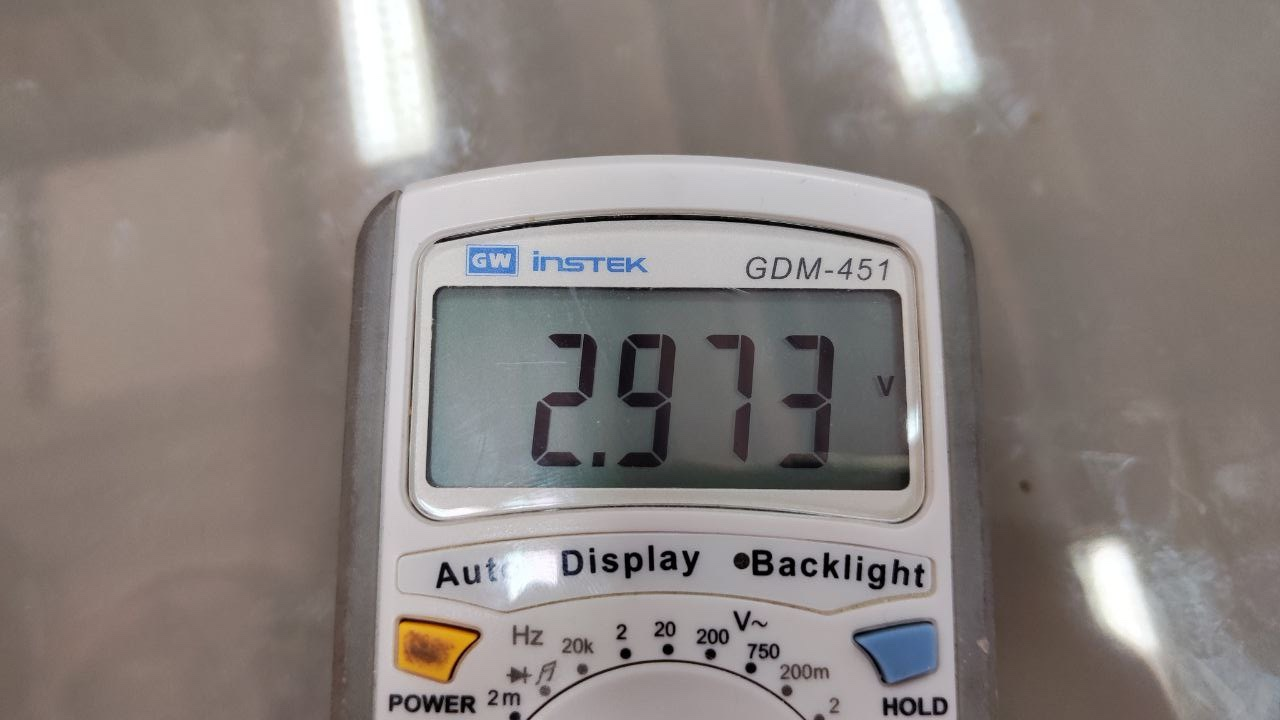
\includegraphics[scale=\PicScale,angle=0]{Fig/26.jpeg}
                \caption{The exact value of $v$ of $R = 2.15k$.}
            \end{figure}

            calculating the power for these two resistors, we have:
            \begin{equation*}
                P_{1k} = \frac{v^2}{R} = \frac{2.06^2}{0.98} = 4.32 \text{ W}
            \end{equation*}
            \begin{equation*}
                P_{2.2k} = \frac{v^2}{R} = \frac{2.97^2}{2.15} = 4.11 \text{ W}
            \end{equation*}
            as can be seen, the power consumed by the $1$ k$\Omega$ resistor is $4.32$ W and
            the power consumed by the $2.2$ k$\Omega$ resistor is $4.11$ W which both are less
            than the maximum power of $4.35$ W.
            So the maximum power transfer theorem is verified.
        }
    \end{subquestion}


\end{question}

\assignmentSection{Bonus Experiments}

%----------------------------------------------------------------------------------------
%	QUESTION 4
%----------------------------------------------------------------------------------------
\begin{question}

    \questiontext{A Zener diode is a special type of diode designed to reliably allow current to flow backwards when a certain set reverse voltage, known as the Zener voltage, is reached. The characteristic curve of a typical Zener diode is shown in Fig. \ref{fig:zener}. Explain how a Zener diode can be used as a voltage source. Is there any practical or analytical limitation on a voltage source created by a Zener diode?}

    \begin{figure}[H]
        \centering
        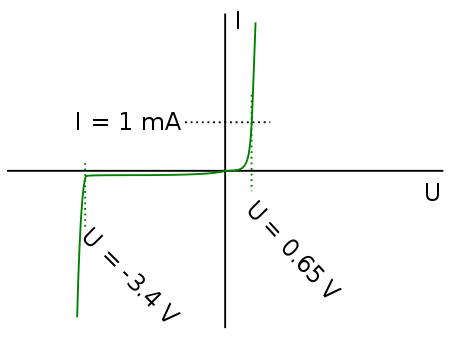
\includegraphics[scale=0.5,angle=0]{Fig/zener.png}
        \caption{Typical characteristic of a Zener diode.} \label{fig:zener}
    \end{figure}

    \answer{
        The Zener diode can be used as a voltage regulator to provide a stable reference
        voltage. This is achieved by operating the Zener diode in its reverse breakdown
        region. When the reverse voltage applied to the Zener diode exceeds
        the Zener breakdown voltage \( V_Z \), the diode conducts and maintains
        a constant voltage \( V_Z \) across its terminals.
        Consider a circuit where a Zener diode is connected in parallel with the
        load resistor \( R_L \) and a series resistor \( R_s \) is placed
        between the supply voltage \( V_s \) and the Zener diode.
        The supply voltage \( V_s \) must be greater than the Zener voltage
        \( V_Z \) for the Zener diode to regulate the voltage.
        The current through the series resistor \( R_s \) is given by:

        \[
            I_s = \frac{V_s - V_Z}{R_s}
        \]

        The current through the load resistor \( R_L \) is:

        \[
            I_L = \frac{V_Z}{R_L}
        \]

        The Zener current \( I_Z \), which is the current flowing through the Zener diode, is:

        \[
            I_Z = I_s - I_L = \frac{V_s - V_Z}{R_s} - \frac{V_Z}{R_L}
        \]

        For proper operation, the Zener current \( I_Z \) must be within the specified limits of the Zener diode. The Zener diode will maintain a constant voltage \( V_Z \) as long as \( I_Z \) remains within these limits.

        There are several practical and analytical limitations to
        consider when using a Zener diode as a voltage source:

        1. \textbf{Power Dissipation:}
        The Zener diode must be able to dissipate the power generated by the Zener current. The power dissipated by the Zener diode \( P_Z \) is:

        \[
            P_Z = V_Z \cdot I_Z
        \]

        Ensure that \( P_Z \) does not exceed the maximum power rating of the Zener diode.

        2. \textbf{Current Limitations:}
        The series resistor \( R_s \) must be chosen to ensure that the Zener current \( I_Z \) remains within the specified operating range of the Zener diode. If the Zener current is too low, the Zener diode may not maintain the voltage regulation. If the Zener current is too high, the diode may overheat and fail.

        3. \textbf{Supply Voltage and Load Variations:}
        The supply voltage \( V_s \) must be sufficiently higher than the Zener voltage \( V_Z \) to maintain regulation. Variations in \( V_s \) can affect the current through the Zener diode and potentially impact voltage regulation.

        4. \textbf{Load Variations:}
        Changes in the load resistance \( R_L \) will affect the load current \( I_L \).
        The series resistor \( R_s \) must be sized to accommodate the expected range of load
        variations while keeping the Zener current \( I_Z \) within the safe operating region. \\

        It's also important to point Zener effect.The Zener effect is
        a type of electrical breakdown that occurs in a reverse biased
        p-n junction when the electric field enables tunneling of
        electrons from the valence to the conduction band of a
        semiconductor, leading to numerous free minority carriers.
        When the reverse voltage applied to the Zener diode reaches
        the Zener voltage, these carriers are accelerated enough to
        create additional carriers through collisions with bound
        electrons, causing a rapid increase in current, while the
        voltage across the diode remains approximately constant.
        This constant voltage,
        even in the face of large changes in current, is what makes the Zener
         diode useful as a voltage regulator. \\

        In summary, a Zener diode can be effectively used as a voltage source to
        provide a stable reference voltage,
        but it is essential to consider power dissipation, current limitations,
        and variations in supply voltage and load to ensure reliable operation.

    }

\end{question}
%----------------------------------------------------------------------------------------
%	QUESTION 5
%----------------------------------------------------------------------------------------

\begin{question}

    \questiontext{Consider the typical characteristic curve of a Zener diode.}
    %---------------------------------------------------------------------------------------
    \begin{subquestion}{Propose a piecewise linear approximation for the characteristic curve using vertical and/or horizontal lines. The forward and (Zener) breakdown voltages should be included in the approximation. }

        \answer{
            To propose a piecewise linear approximation for the characteristic curve of a Zener diode, we can approximate the curve using vertical and horizontal lines that represent the forward and breakdown voltages. The key points to consider are the forward voltage \( V_F \) and the Zener breakdown voltage \( V_Z \).

            1. \textbf{Forward Bias Region:}
            - For \( U > V_F \), the diode conducts and we approximate it with a horizontal line at the forward voltage \( V_F \) (typically 0.7V for a silicon diode).

            2. \textbf{Reverse Breakdown Region:}
            - For \( U < -V_Z \), the Zener diode enters breakdown and we approximate it with a horizontal line at the Zener voltage \( V_Z \) (e.g., -10V).

            3. \textbf{Non-Conducting Region:}
            - For \( -V_Z < U < V_F \), the diode does not conduct, and we approximate it with a vertical line at zero current.

            The piecewise linear approximation can be expressed as:
            \[
                I(U) =
                \begin{cases}
                    I_{F}  & \text{for } U \geq V_F     \\
                    0      & \text{for } -V_Z < U < V_F \\
                    -I_{Z} & \text{for } U \leq -V_Z
                \end{cases}
            \]

            Where \( I_F \) is the current in the forward bias and \( I_Z \) is the Zener current in breakdown.

        }

    \end{subquestion}

    %----------------------------------------------------------------------------------------
    \begin{subquestion}{Use the proposed piecewise linear approximation to suggest a model for the Zener diode. You may use ideal diodes, independent sources, or passive LTI resistors in your model. }

        \answer{
            Using the piecewise linear approximation from part (a), we can suggest a model for the Zener diode using ideal diodes, independent sources, and passive LTI resistors.

            1. \textbf{Forward Bias Model:}
            - An ideal diode in series with a voltage source \( V_F \) (0.7V) represents the forward bias region.

            2. \textbf{Reverse Breakdown Model:}
            - An ideal diode in series with a voltage source \( V_Z \) (-10V) represents the breakdown region. This series combination is placed in parallel with the forward bias model.

            3. \textbf{Non-Conducting Region:}
            - This region is represented by an open circuit (no current flow).

            The equivalent circuit model for the Zener diode is thus composed of:
            - An ideal diode \( D_1 \) in series with a voltage source \( V_F \).
            - A second ideal diode \( D_2 \) in series with a voltage source \( V_Z \) placed in reverse bias.

            The model can be represented as:

            \[
                \begin{cases}
                    D_1 + V_F & \text{for forward bias}      \\
                    D_2 + V_Z & \text{for reverse breakdown}
                \end{cases}
            \]

            Where \( D_1 \) and \( D_2 \) are ideal diodes.
        }

    \end{subquestion}

    %----------------------------------------------------------------------------------------
    \begin{subquestion}{Use PSpice simulation to verify the accuracy of the suggested model for D02CZ10 zener diode with the forward and breakdown voltages around $0.7$ and $-10$ V. }

        \answer{To verify the accuracy of the suggested model for the D02CZ10 Zener diode with forward and breakdown voltages around 0.7V and -10V, respectively, we can use PSpice simulation.


            The model in PSpice looks like:
            \begin{figure}[H]
                \centering
                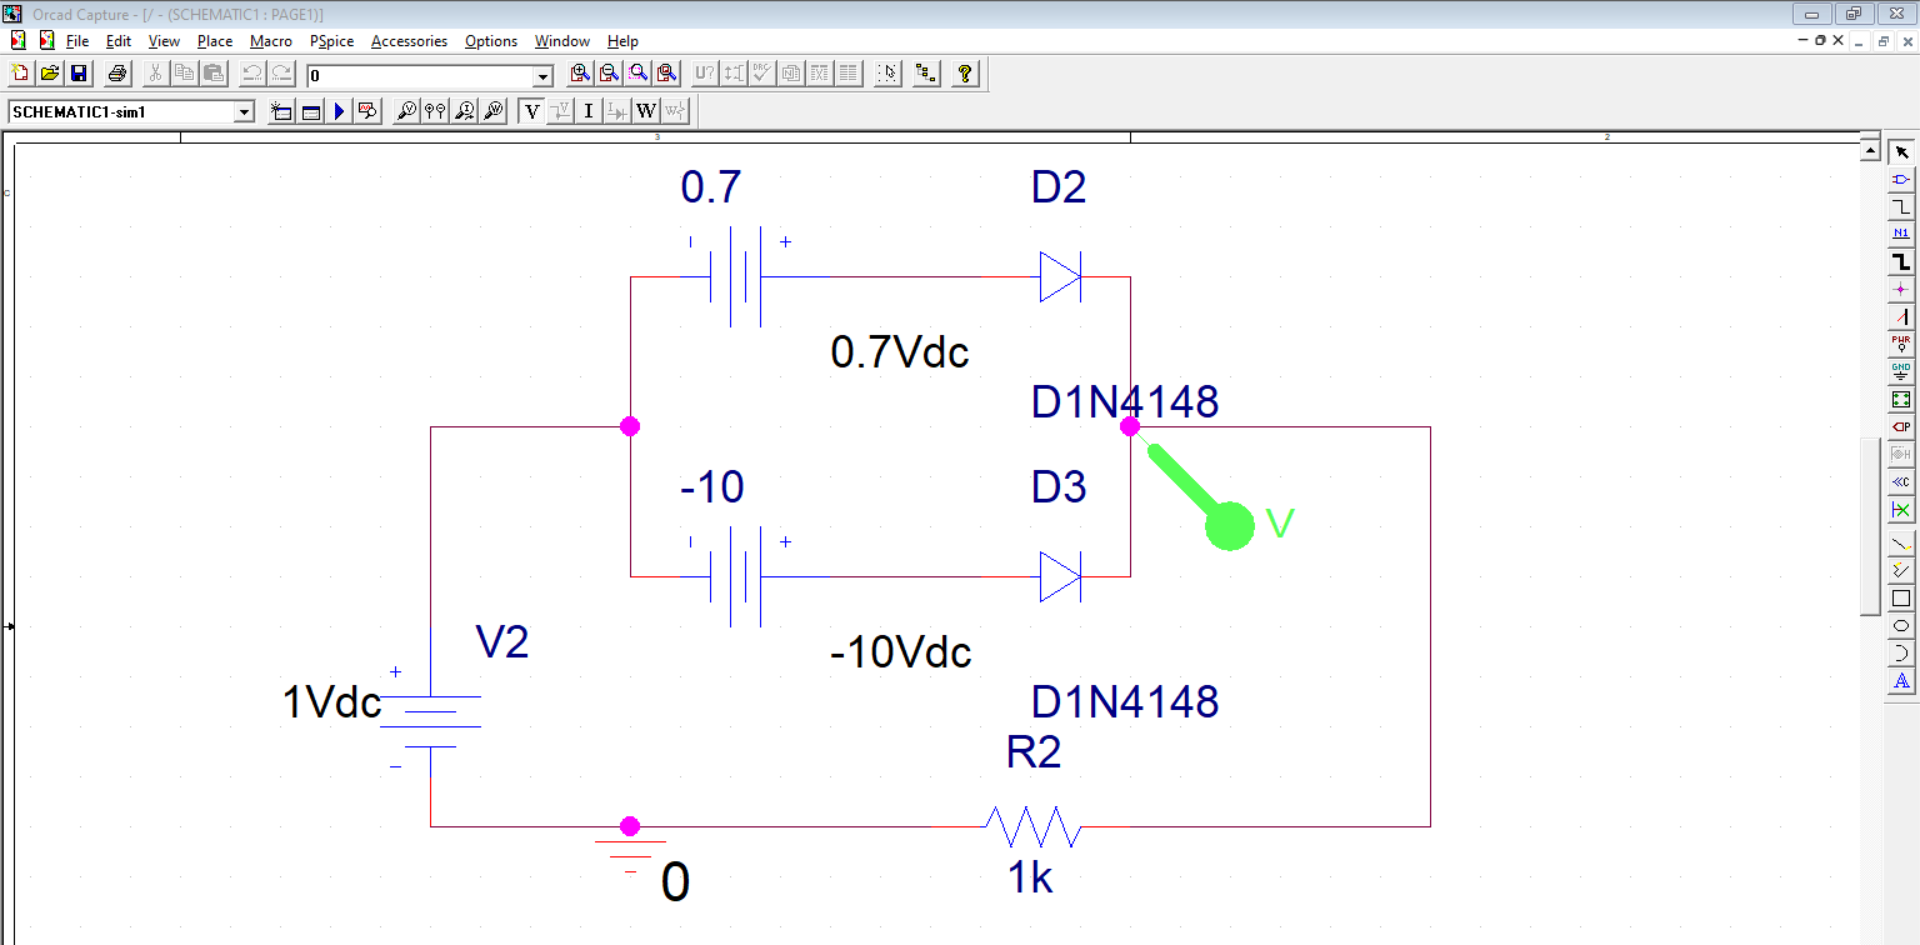
\includegraphics[scale=0.35,angle=0]{Fig/Q5_1.png}
                \caption{circuit in PSpice}
            \end{figure}

            and here is the output of the simulation:
            \begin{figure}[H]
                \centering
                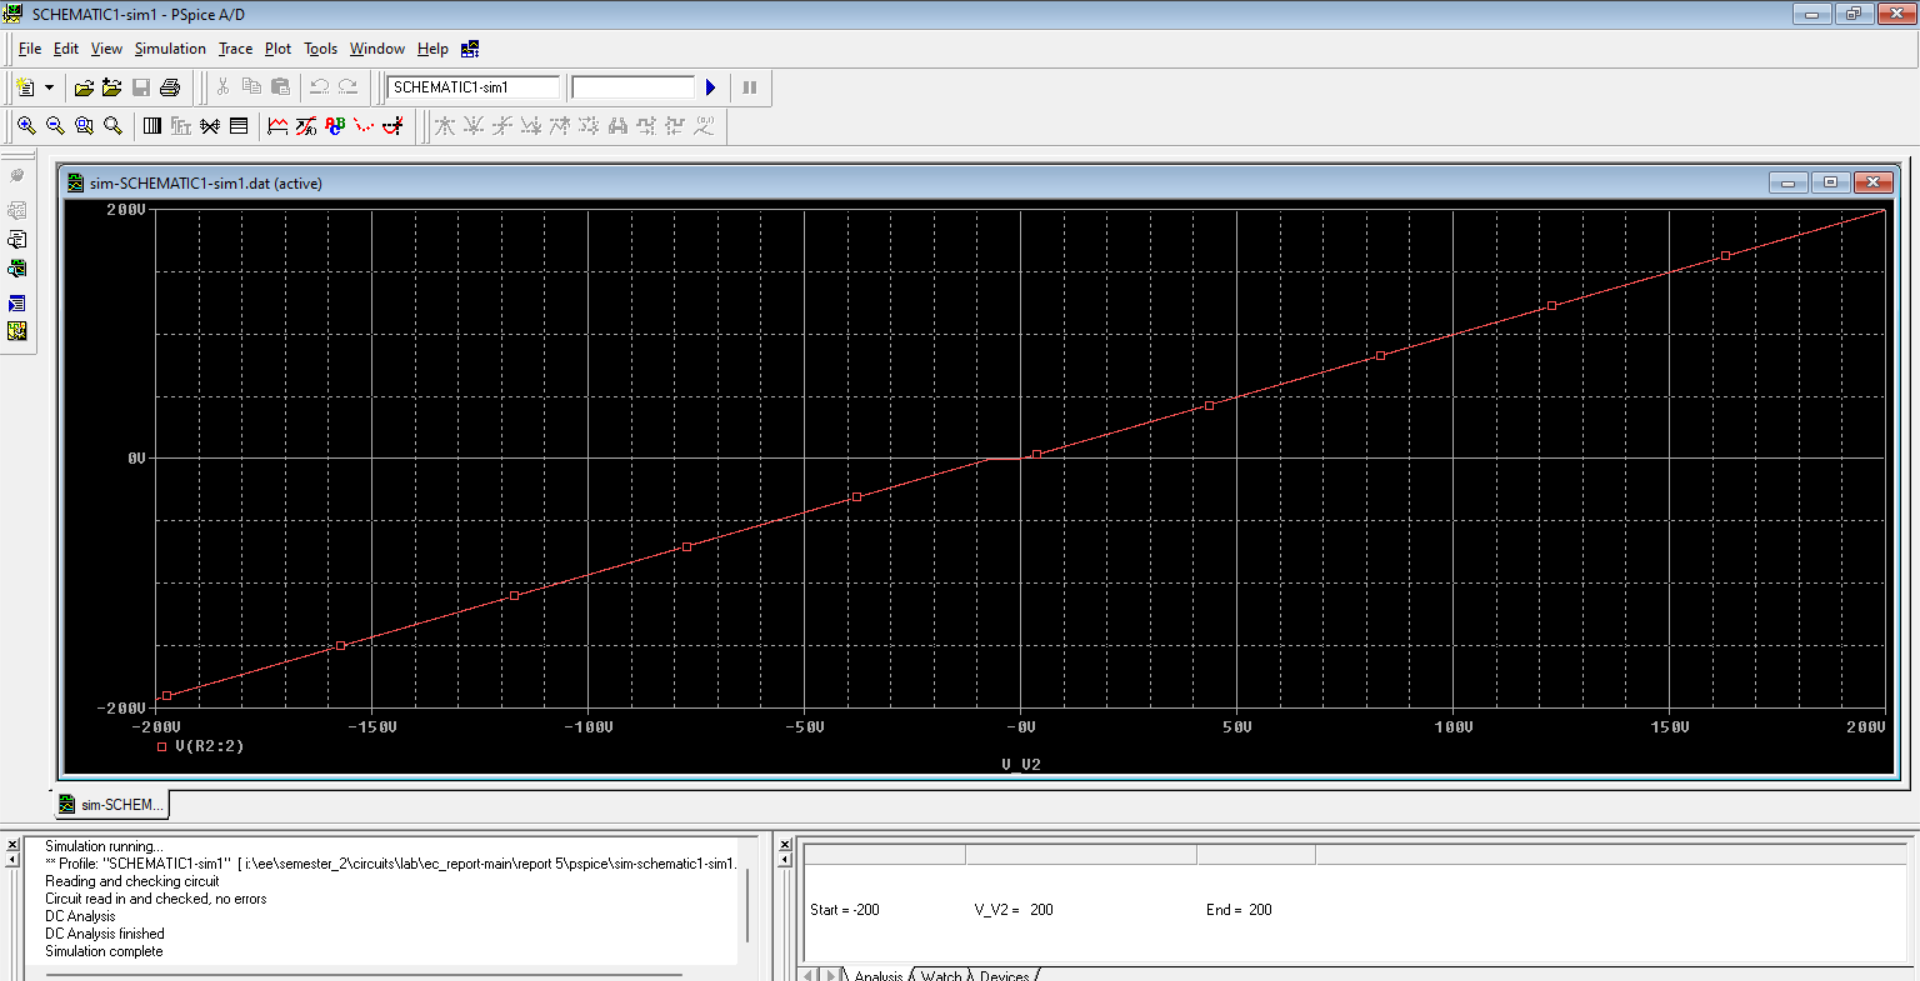
\includegraphics[scale=0.35,angle=0]{Fig/Q5_2.png}
                \caption{simulation results}
            \end{figure}

            Also, here is the desired Matlab code for the simulation:
            \lstinputlisting[style=Matlab-Pyglike]{code/one.m}
            

        }

    \end{subquestion}

\end{question}



%----------------------------------------------------------------------------------------
%	QUESTION 6
%----------------------------------------------------------------------------------------

\begin{question}

    \questiontext{Return your work report by filling the \LaTeX template of the manual. Include useful and high-quality images to make the report more readable and understandable.}

\end{question}

%----------------------------------------------------------------------------------------

\end{document}
